\documentclass{article}

\usepackage[margin=1.00in]{geometry}

\usepackage{amsmath}
\usepackage{amsfonts}
\usepackage{graphicx}

\usepackage{xcolor}
\usepackage{listings}
\colorlet{mygray}{black!30}
\colorlet{mygreen}{green!60!blue}
\colorlet{mymauve}{red!60!blue}

\lstset{
  backgroundcolor=\color{gray!10},
  basicstyle=\ttfamily,
  columns=fullflexible,
  breakatwhitespace=false,
  breaklines=true,
  captionpos=b,
  commentstyle=\color{mygreen},
  extendedchars=true,
  frame=single,
  keepspaces=true,
  keywordstyle=\color{blue},
  language=c++,
  numbers=none,
  numbersep=5pt,
  numberstyle=\tiny\color{blue},
  rulecolor=\color{mygray},
  showspaces=false,
  showtabs=false,
  stepnumber=5,
  stringstyle=\color{mymauve},
  tabsize=3,
  title=\lstname
}
%\lstset { %
%    language=C++,
%    backgroundcolor=\color{black!5}, % set backgroundcolor
%    basicstyle=\footnotesize,% basic font setting
%}



\newcommand{\dv}{\mathrm{div}\ }
\newcommand{\curl}{\mathrm{curl}\ }
\newcommand{\grad}{\triangledown}
\newcommand{\R}{\mathbb{R}\ }

\begin{document}

\title{MHD}
\author{Bryn Barker}
\date{May 5, 2021}

\maketitle

\section*{Big Picture}
Magnetohydrodynamics (MHD) couples the Navier-Stokes equations for fluid dynamics with Maxwell's equation of electromagnetism to describe the behavior of conducting fluids, such as plasmas.
The main concept behind MHD is that magnetic fields can induce currents in a moving conductive fluid,
which in turn create forces on the fluid and affect the magnetic field itself \cite{ASThesis}. %cite = xhttps://www.numa.uni-linz.ac.at/Teaching/Bachelor/schafelner-bakk.pdf
Research in MHD waves is a driving force in developing an experimental tokamak nuclear fusion reactor which has huge potential impacts in power generation.

There are various physical applications of MHD that correpsond to both incompressible and compressible gases. The eventual goal of this project is to create a finite element simulation of 2D compressible MHD that can be used to verify analytic stability results developed in \cite{bryn}. However, due to the fact that compressibility greatly complicates the system, we will begin with an incompressible MHD solver and leave the compressible solver as a future extension of this code. 

We will make one additional key simplification here which is that we will not include the conservation of energy in the Navier-Stokes equations in our MHD system. Solving for temperature in addition to the other relevant quantities complicates the solver and thus we will leave this part of the model as another future extension of the code. 

In vector notation, the simplified equations of 2D incompressible MHD are given in Eulerian coordinates by
\begin{align*}
    \nabla \cdot \boldsymbol{u} &= 0,\\
    \rho \frac{\partial  \boldsymbol{u}}{\partial t} + \rho \boldsymbol{u} \cdot \nabla \boldsymbol{u} + \nabla p &= \mu \Delta \boldsymbol{u}+ \left(\boldsymbol{h}\cdot \nabla \boldsymbol{h} - \frac{1}{2}\nabla \boldsymbol{h}^2\right),\\
    \frac{\partial \boldsymbol{h} }{\partial t} - \nabla \times (\boldsymbol{u}\times \boldsymbol{h}) &= -\nu \nabla \times (\nabla \times \boldsymbol{h}), \\
    -\nabla \cdot \boldsymbol{h} &= 0,
\end{align*}

where the first two equations correspond to the Navier-Stokes flow and the last two equations correspond to the magnetic field governed by Maxwell's equations. The coupling takes place in the fluid velocity in Maxwell's equations and the forcing term in the Navier-Stokes equations. 

As mentioned, the end goal is to compare this model to the stability results developed in \cite{bryn}. In this work, we use the Evans function to determine the spectral stability of traveling wave solutions of the code. In order to guarentee this method works, we must have consistent splitting of the basis corresponding to the solution on the unstable and stable manifolds. This is accomplished by using the $\beta$-model of the system which is given below. More details can be found in \cite{BMZ}.
\begin{align*}
    \nabla \cdot \boldsymbol{u} &= 0,\\
    \rho \frac{\partial  \boldsymbol{u}}{\partial t} + \rho \boldsymbol{u} \cdot \nabla \boldsymbol{u} + \nabla p &= \mu \Delta \boldsymbol{u}+ \left(\boldsymbol{h}\cdot \nabla \boldsymbol{h} - \frac{1}{2}\nabla \boldsymbol{h}^2\right),\\
    \frac{\partial \boldsymbol{h} }{\partial t} - \nabla \times (\boldsymbol{u}\times \boldsymbol{h}) &=- \beta (\nabla \cdot \boldsymbol{h})\boldsymbol{e}_1 -\nu \nabla \times (\nabla \times \boldsymbol{h}), \\
    -\nabla \cdot \boldsymbol{h} &= 0,
\end{align*}

Lastly, notice that in these six equations we only have five unknowns: two magnetic field components, two velocity components, and pressure. So our system is over determined, and more specifically it is the Maxwell equations that are over determined. To compensate for this, we will add a lagrange multiplier field ($q$) to the Maxwell equations which will inforce the divergence free condition. We will set this lagrange field to be zero on the domain boundary and thus its exact solution is zero. This means that adding this term to the matrix will not affect the continuous solution. 
\begin{align*}
    \nabla \cdot \boldsymbol{u} &= 0,\\
    \rho \frac{\partial  \boldsymbol{u}}{\partial t} + \rho \boldsymbol{u} \cdot \nabla \boldsymbol{u} + \nabla p &= \mu \Delta \boldsymbol{u}+ \left(\boldsymbol{h}\cdot \nabla \boldsymbol{h} - \frac{1}{2}\nabla \boldsymbol{h}^2\right),\\
    \frac{\partial \boldsymbol{h} }{\partial t} - \nabla \times (\boldsymbol{u}\times \boldsymbol{h}) +\nabla q &=- \beta (\nabla \cdot \boldsymbol{h})\boldsymbol{e}_1 -\nu \nabla \times (\nabla \times \boldsymbol{h}), \\
    -\nabla \cdot \boldsymbol{h} &= 0,
\end{align*}

Now that we have defined the full MHD system, we will break the problem down and show how to solve it. We will write two separate solvers, one for the Maxwell's equations and one for the incompressible Navier-Stokes. Then we will couple the two solvers together. 

\section*{Maxwell System}
The Maxwell's equations relevant to MHD are given by
\begin{align*}
    \frac{\partial \boldsymbol{h} }{\partial t} - \nabla \times (\boldsymbol{u}\times \boldsymbol{h}) +\nabla q &=- \beta (\nabla \cdot \boldsymbol{h})\boldsymbol{e}_1 -\nu \nabla \times (\nabla \times \boldsymbol{h}), \\
    -\nabla \cdot \boldsymbol{h} &= 0,
\end{align*}
along with the Lorenz force which acts as the forcing function in the Navier-Stokes equations and is given by
\[
    \boldsymbol{f}_L =  \boldsymbol{h}\cdot \nabla \boldsymbol{h} - \frac{1}{2}\nabla \boldsymbol{h}^2.
\]
The Lorenz force is not relevant in the Maxwell solver but will come up later. 
This simplified Maxwell system given is comprised of the induction equation with the modifications which we mentioned above, and the divergence free condition. Since we are only considering the uncoupled Maxwell equations right now, we will treat $\boldsymbol{u}$ as a constant velocity field for the time being. 

Now in order to test this solver with the method of manufactured solutions, we will add a forcing function to the right hand side of the induction equation in this system, yielding, 
\begin{align*}
    \frac{\partial \boldsymbol{h} }{\partial t} - \nabla \times (\boldsymbol{u}\times \boldsymbol{h}) +\nabla q &=- \beta (\nabla \cdot \boldsymbol{h})\boldsymbol{e}_1 -\nu \nabla \times (\nabla \times \boldsymbol{h}) + \boldsymbol{f}, \\
    -\nabla \cdot \boldsymbol{h} &= 0,
\end{align*}

In order to obtain the weak form of this systme, let's first express the current system in vector form as
\[
    \begin{bmatrix} \frac{\partial \boldsymbol{h} }{\partial t} - \nabla \times (\boldsymbol{u}\times \boldsymbol{h}) + \nu \nabla \times (\nabla \times \boldsymbol{h}) + \nabla q + \beta (\nabla \cdot \boldsymbol{h})\boldsymbol{e}_1 \\ \nabla \cdot \boldsymbol{h} \end{bmatrix} = \begin{bmatrix} \boldsymbol{f} \\ 0 \end{bmatrix}.
    \]
    Next, we take the dot product from the left with the vector-valued test function $\phi = \begin{bmatrix} \boldsymbol{v} \\ w \end{bmatrix}$ and integrate over the domain $\Omega$ to obtain the following,
        \[
            \left(\boldsymbol{v},\frac{\partial \boldsymbol{h} }{\partial t} - \nabla \times (\boldsymbol{u}\times \boldsymbol{h}) + \nu \nabla \times (\nabla \times \boldsymbol{h}) + \nabla q + \beta (\nabla \cdot \boldsymbol{h})\boldsymbol{e}_1 \right)_\Omega - \left(w,\nabla  \cdot \boldsymbol{h}\right)_\Omega = (\boldsymbol{v},\boldsymbol{f})_\Omega,
        \]
        or equivalently, 
        \[
            \left(\boldsymbol{v},\frac{\partial \boldsymbol{h} }{\partial t}\right)_\Omega
            -\left(\boldsymbol{v},\nabla \times (\boldsymbol{u}\times \boldsymbol{h})\right)_\Omega
            + \nu\left(\boldsymbol{v},\nabla \times (\nabla \times \boldsymbol{h})\right)_\Omega
            + \left(\boldsymbol{v},\nabla q\right)_\Omega
            + \beta\left(\boldsymbol{v}, (\nabla \cdot \boldsymbol{h})\boldsymbol{e}_1\right)_\Omega
            -\left(w,\nabla  \cdot \boldsymbol{h}\right)_\Omega = (\boldsymbol{v},\boldsymbol{f})_\Omega.
        \]
        Now applying integration by parts to the higher order terms on the left hand side we get
        \begin{align*}
            \left(\boldsymbol{v},\frac{\partial \boldsymbol{h} }{\partial t}\right)_\Omega
            -\left(\nabla \times \boldsymbol{v},\boldsymbol{u}\times \boldsymbol{h}\right)_\Omega
            +\left(\boldsymbol{v}\times\boldsymbol{n},\boldsymbol{u}\times \boldsymbol{h}\right)_\Gamma
            + \nu\left(\nabla \times\boldsymbol{v},\nabla \times \boldsymbol{h}\right)_\Omega
            -\nu\left(\boldsymbol{v}\times\boldsymbol{n},\nabla \times \boldsymbol{h}\right)_\Gamma &\\
            - \left(\nabla \cdot \boldsymbol{v},q\right)_\Omega
            +\left(\boldsymbol{n}\cdot \boldsymbol{v},p\right)_\Gamma
            + \beta\left(\boldsymbol{v}, (\nabla \cdot \boldsymbol{h})\boldsymbol{e}_1\right)_\Omega
            -\left(w,\nabla  \cdot \boldsymbol{h}\right)_\Omega &= (\boldsymbol{v},\boldsymbol{f})_\Omega,
        \end{align*}
        which simplifies to
        \[
            \left(\boldsymbol{v},\frac{\partial \boldsymbol{h} }{\partial t}\right)_\Omega
            -\left(\nabla \times \boldsymbol{v},\boldsymbol{u}\times \boldsymbol{h}\right)_\Omega
            + \nu\left(\nabla \times\boldsymbol{v},\nabla \times \boldsymbol{h}\right)_\Omega
            - \left(\nabla \cdot \boldsymbol{v},q\right)_\Omega
            + \beta\left(\boldsymbol{v}, (\nabla \cdot \boldsymbol{h})\boldsymbol{e}_1\right)_\Omega
            -\left(w,\nabla  \cdot \boldsymbol{h}\right)_\Omega = (\boldsymbol{v},\boldsymbol{f})_\Omega.
        \]

        Finally, it remains to discretize our time derivative of the magnetic field. We will do this with a simple backward Euler approximation
        \begin{align*}
            \left(\boldsymbol{v},\boldsymbol{h}^{n+1} \right)_\Omega
            -\Delta t (\nabla \times   \boldsymbol{v},&\boldsymbol{u}\times \boldsymbol{h}^{n+1})_\Omega
            +\Delta t \nu\left(\nabla \times\boldsymbol{v},\nabla \times \boldsymbol{h}^{n+1}\right)_\Omega
            - \Delta t \left(\nabla \cdot \boldsymbol{v},q^{n+1}\right)_\Omega \\
            &+ \Delta t \beta\left(\boldsymbol{v}, (\nabla \cdot \boldsymbol{h}^{n+1})\boldsymbol{e}_1\right)_\Omega
            -\Delta t\left(w,\nabla  \cdot \boldsymbol{h}^{n+1}\right)_\Omega = \left(\boldsymbol{v},\boldsymbol{h}^{n}\right)_\Omega +\Delta t (\boldsymbol{v},\boldsymbol{f}^{n+1})_\Omega,
        \end{align*}
        where $\Delta t$ is the time step size.


        As a result of the third term on the left hand side of the weak form, we want to use $H(curl)$ conforming elements for the magnetic field. Meaning essentially that we want the curl of the shape functions defining the magnetic field to be integrable in the $L^2$ norm. Fortunately, there is a well known finite element that satisfies this property: namely the Nedelec element. These elements are only guarenteed to be continuous in the tangential component. 

        As a quick note, we see that in our weak form, the velocity field is used to construct our system matrix. As a result, when we couple the systems and velocity is no longer constant, the system matrix will need to be updated at each time step. In an effort to reduce computational complexity, as a future step it might be worth looking into using an IMEX method instead of backward Euler and moving the term with the velocity field to the right hand side of the system. This would also result in a symmetric system matrix.

        We still need to specify boundary conditions. For the time being we will assume the magnetic field has Dirichlet boundary conditions on the entire domain boundary $\Gamma$ and by construction we choose the lagrange multiplier to have zero boundary conditions on the entire domain boundary. These conditions are given by
        \[
            \boldsymbol{h} = \boldsymbol{g} \text{ on } \Gamma,\quad \quad q = 0 \text{ on } \Gamma,
        \]
        for some vector valued function $\boldsymbol{g}$.

        Now let's discretize in space. As mentioned, we will use $H(curl)$ conforming Nedelec elements for the magnetic field and standard Lagrangian finite elements for the lagrange multiplier. With this we will define the following discrete function spaces,
        \[
            \boldsymbol{V}_g = \{\boldsymbol{\phi}\in H(curl;\Omega) | \boldsymbol{\phi}_\Gamma = \boldsymbol{g}\},\quad
            \boldsymbol{V}_0 = \{\boldsymbol{\phi}\in H(curl;\Omega) | \boldsymbol{\phi}_\Gamma = 0\},\quad
            Q_0 = \{\phi \in L^2(\Omega) | \phi_\Gamma = 0\},
        \]

        With this, our variational formulation of the problem is written as: given $\boldsymbol{h}^0 =\boldsymbol{h}(t=0)$, for each time step $n$, find $\boldsymbol{h}^{n+1} \in \boldsymbol{V}_g$ and $q^{n+1} \in Q_0$ such that for all $\boldsymbol{v} \in \boldsymbol{V}_0$ and $w \in Q_0$
        \begin{align*}
            \left(\boldsymbol{v},\boldsymbol{h}^{n+1} \right)_\Omega
            -\Delta t (\nabla \times   \boldsymbol{v},&\boldsymbol{u}\times \boldsymbol{h}^{n+1})_\Omega
            +\Delta t \nu\left(\nabla \times\boldsymbol{v},\nabla \times \boldsymbol{h}^{n+1}\right)_\Omega
            - \Delta t \left(\nabla \cdot \boldsymbol{v},q^{n+1}\right)_\Omega \\
            &+ \Delta t \beta\left(\boldsymbol{v}, (\nabla \cdot \boldsymbol{h}^{n+1})\boldsymbol{e}_1\right)_\Omega
            -\Delta t\left(w,\nabla  \cdot \boldsymbol{h}^{n+1}\right)_\Omega = \left(\boldsymbol{v},\boldsymbol{h}^{n}\right)_\Omega +\Delta t (\boldsymbol{v},\boldsymbol{f}^{n+1})_\Omega.
        \end{align*}


        This system is a saddle point problem and thus must be set up to satisfy the inf-sup stablity condition. This is achieved by setting the degree of the Nedelec elements to be one higher than the degree of the Lagrangian elements for the lagrange multiplier.

        We can express this system with the following block matrix system,
        \[ \begin{bmatrix} A & B^\top \\ B & 0 \end{bmatrix} \begin{bmatrix} H \\ Q \end{bmatrix} = \begin{bmatrix} F \\ 0 \end{bmatrix}, \]
            where $A$ is composed of the mass matrix, the velocity term, the curl-curl operator, and the beta term. $B$ is the negative divergence operator, with its transpose being the gradient operator. And $F$ is the mass matrix times the previous magnetic field and the forcing function.

            We will use the Schur decomposition to solve this sytem in two steps
            \begin{align*}
                BA^{-1}B^T &Q = BA^{-1}F \\
                A H =& F - BQ.
            \end{align*}
            To solve this system we are essentially inverting the Schur complement of $A$, which is $BA^{-1}B^T$ and the matrix $A$ itself. Due to the nature of $A$, we will use a direct LU decomposition to solve for the inverse of $A$. And for the Schur complement, we will use a nonsymmetric solver (GMRES) and a preconditioner to invert the system. Since this is a saddle point problem, a good choice for a preconditioner is the inverse of the mass matrix associated with the lagrange multiplier. To invert the mass matrix we will also use an iterative method preconditioned with an SSOR preconditioner initialized with the mass matrix. 

            And that's a wrap on the Maxwell Solver! We will look more closely at the code for the Maxwell Solver after discussing the Navier-Stokes solver. 

            \subsection*{Testing the Maxwell Solver}
            To start, I tested the solver on constant, linear, and quadratic exact solutions to ensure it functioned as expected and sure enough the solver was able to solve these test problems exactly up to machine precision. So to test the convergence, I used the following more complicated test problem,
            \[ \begin{bmatrix} \boldsymbol{h} \\ q\end{bmatrix} = \begin{bmatrix} t \cos(y) \\ t \sin(y) \\ 0 \end{bmatrix}.\]
                The approximated solution for the magnetic field in the $x$-component is shown in the figure below.

                \begin{center}
                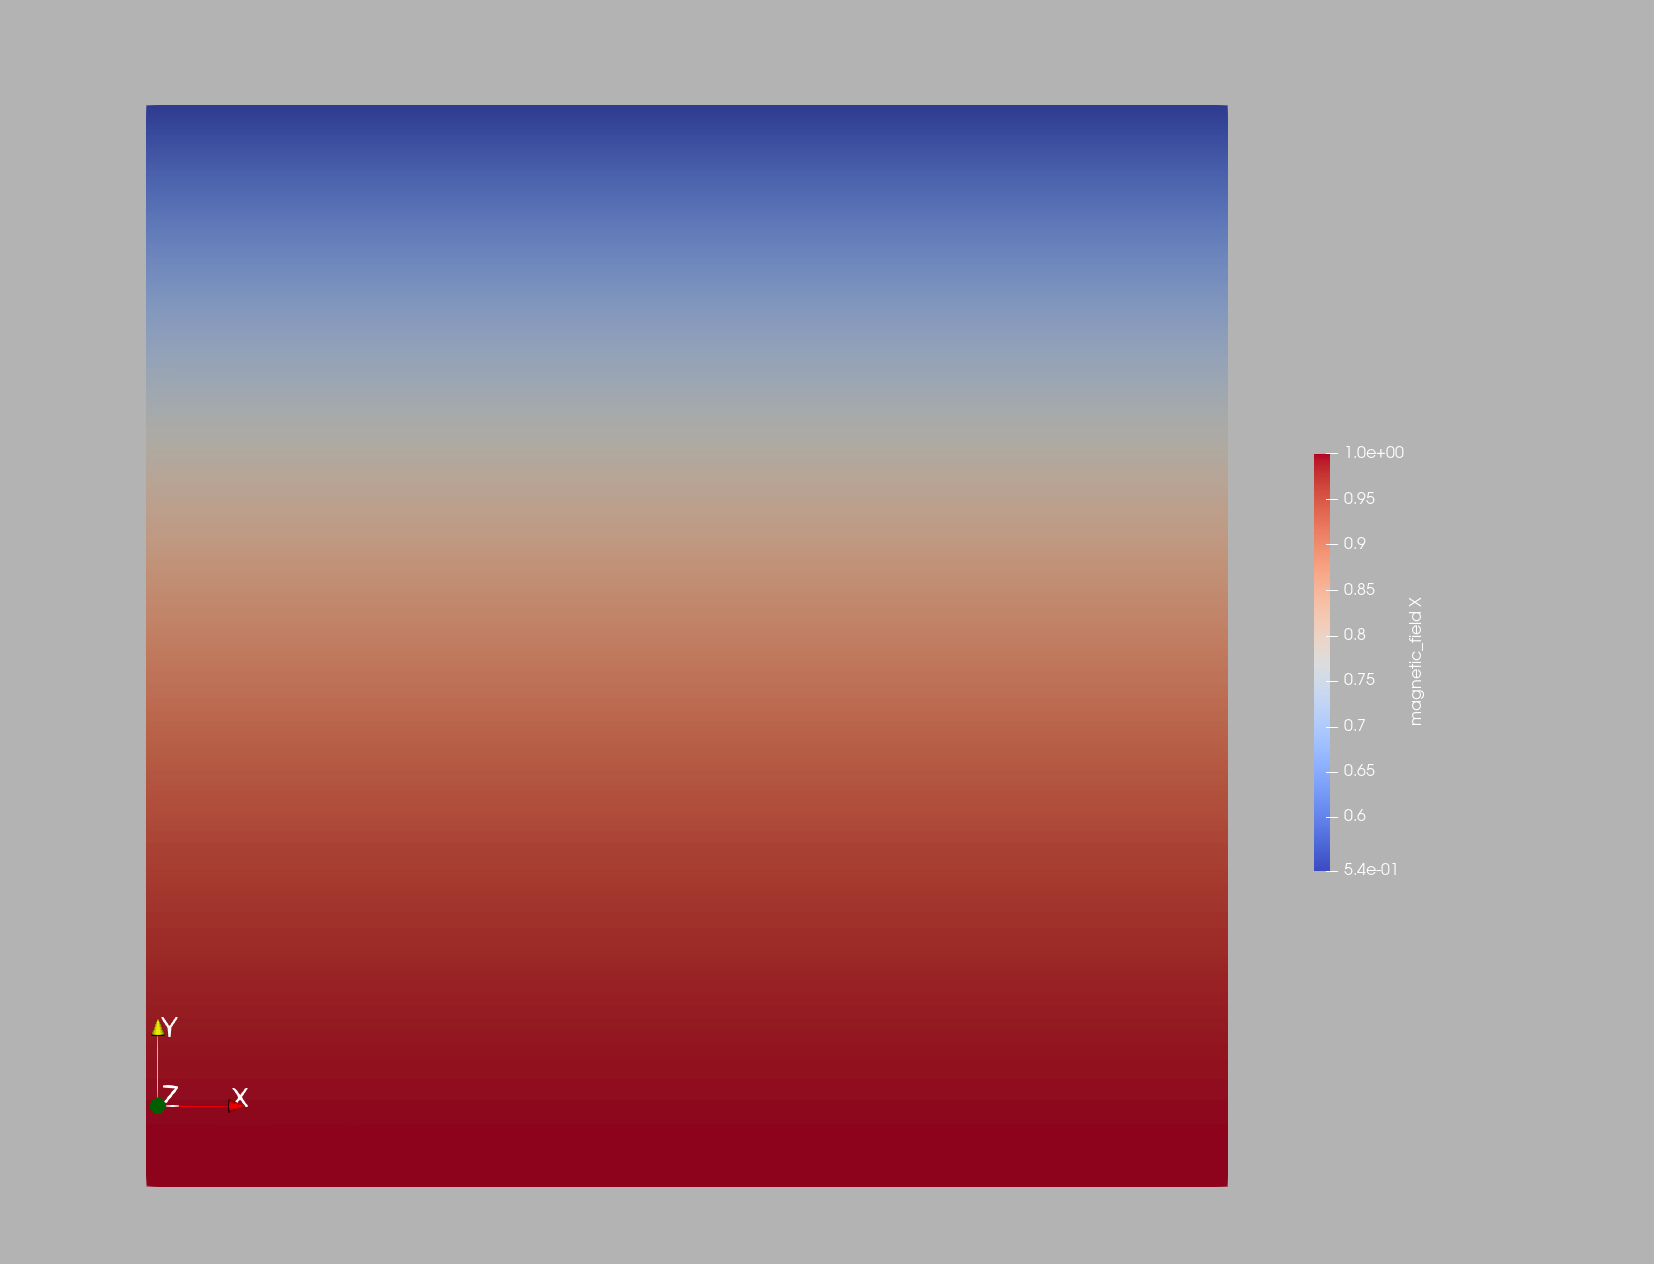
\includegraphics[scale=.2]{mag_x.png}
                \end{center}

                And the magnetic field in the $y$-component:

                \begin{center}
                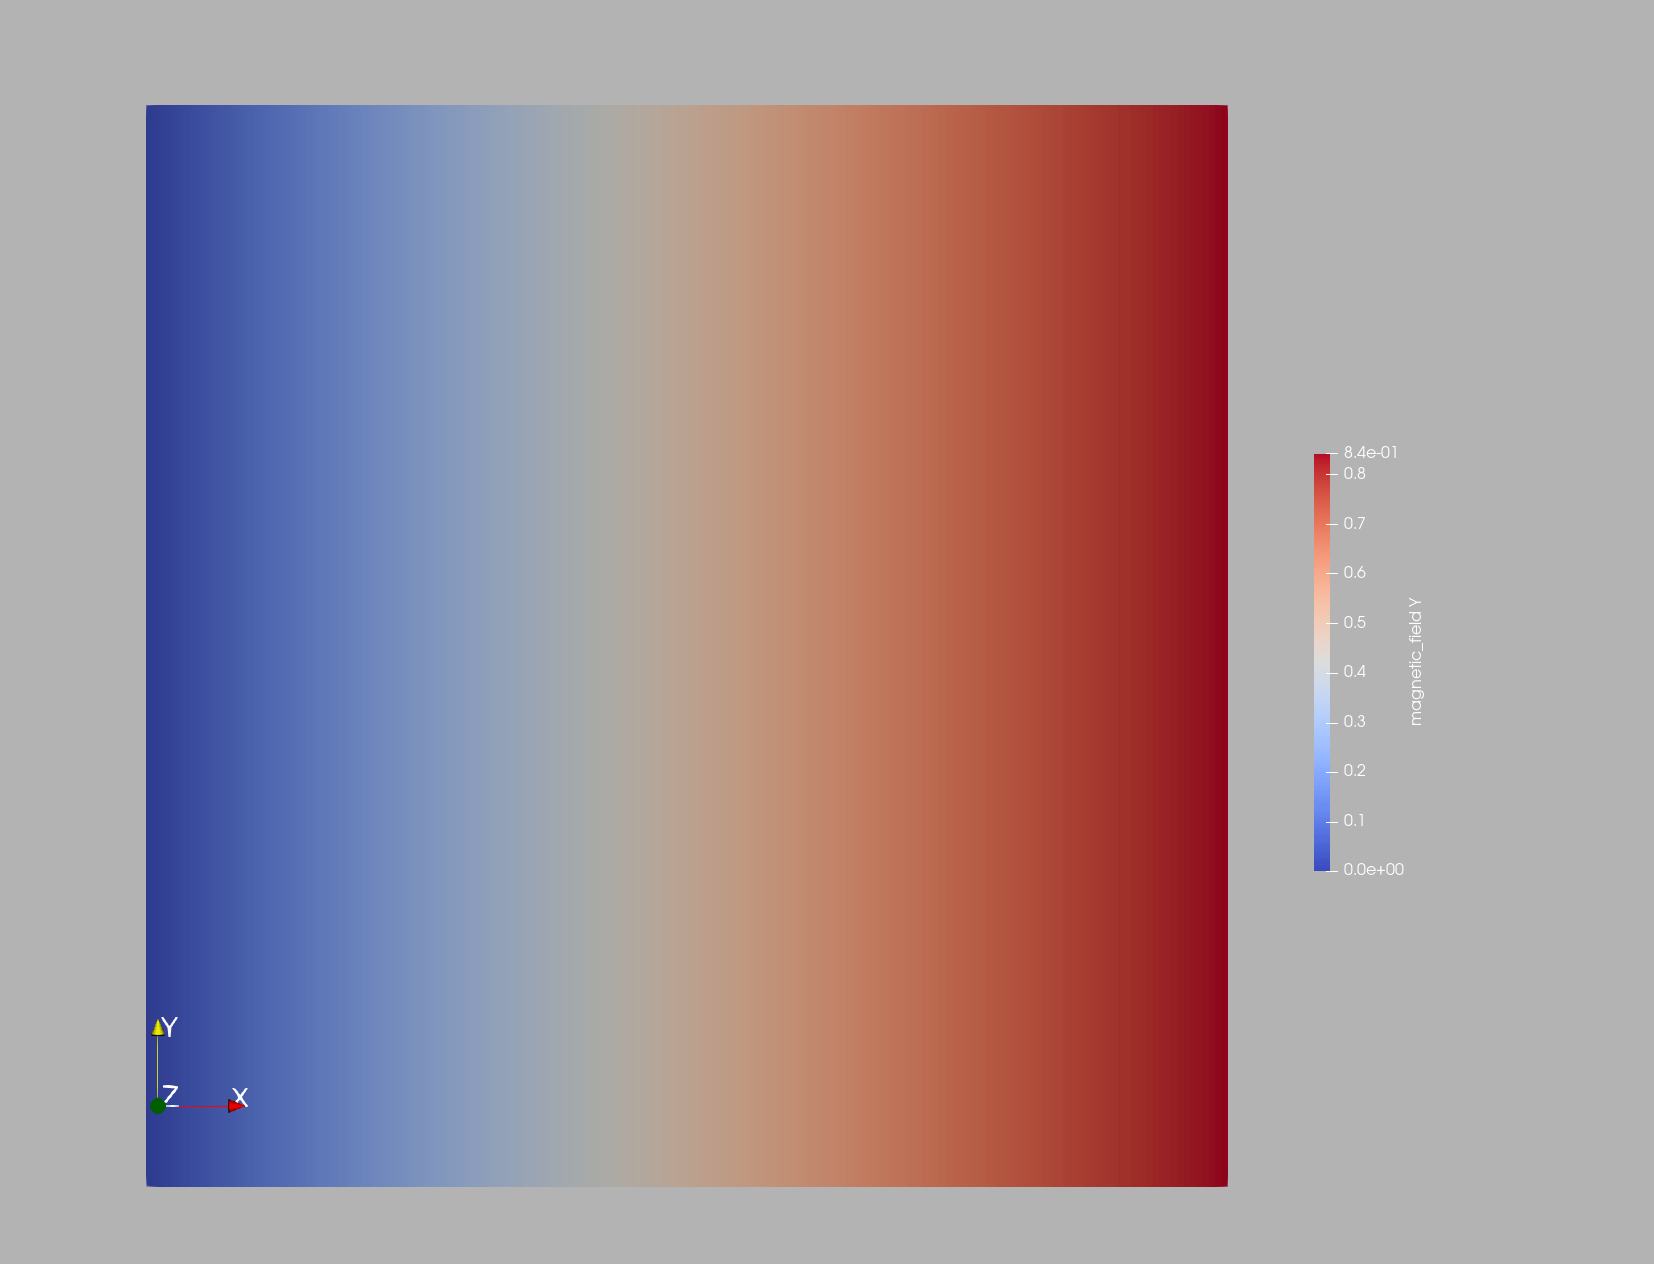
\includegraphics[scale=.2]{mag_y.png}
                \end{center}

                Finally, the solution to the lagrange multiplier, which we hope to be uniformly zero:

                \begin{center}
                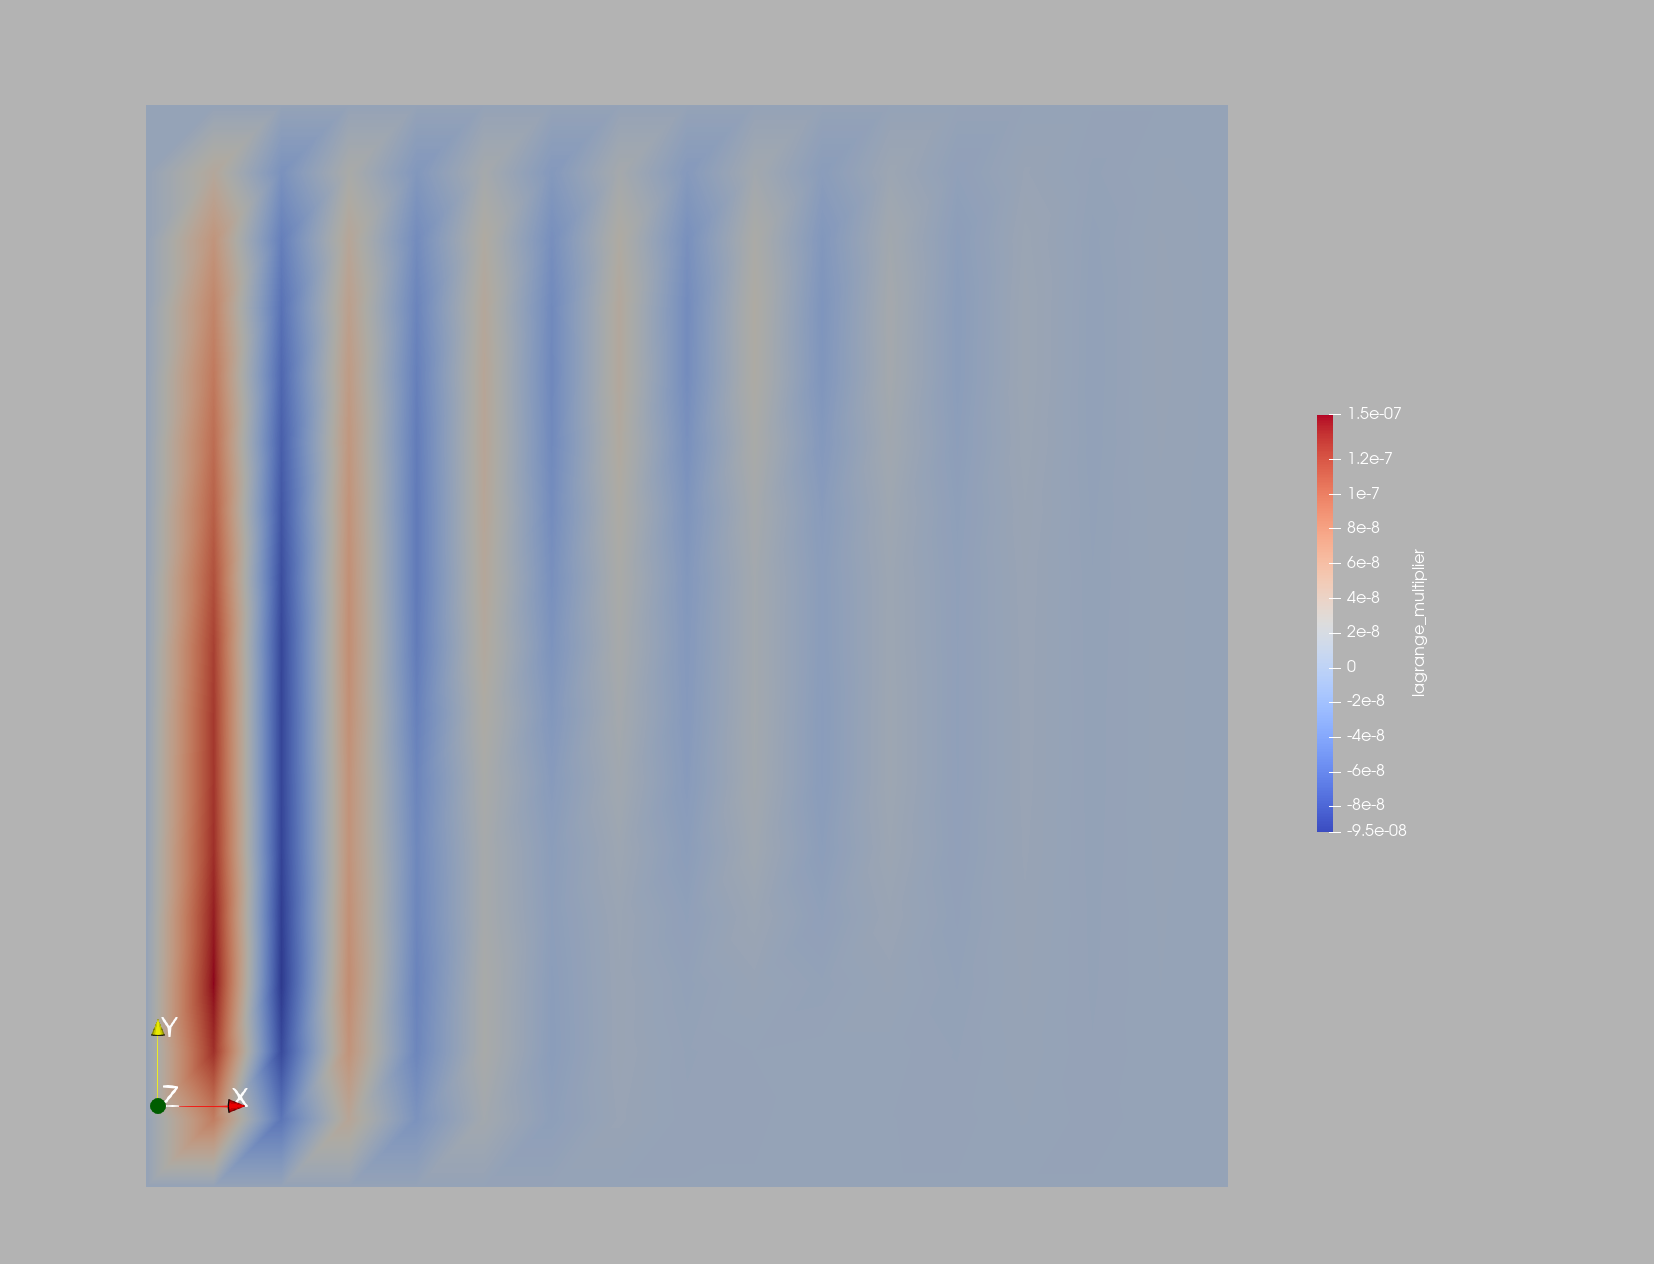
\includegraphics[scale=.2]{lagrange.png}
                \end{center}

                The results were as hoped, notice the scaling on the lagrange multiplier shows that the solution is quite uniform despite the irregular pattern shown. The following graph shows the convergence results for the three components combined based on the $L^\infty$ norm.

                \begin{center}
                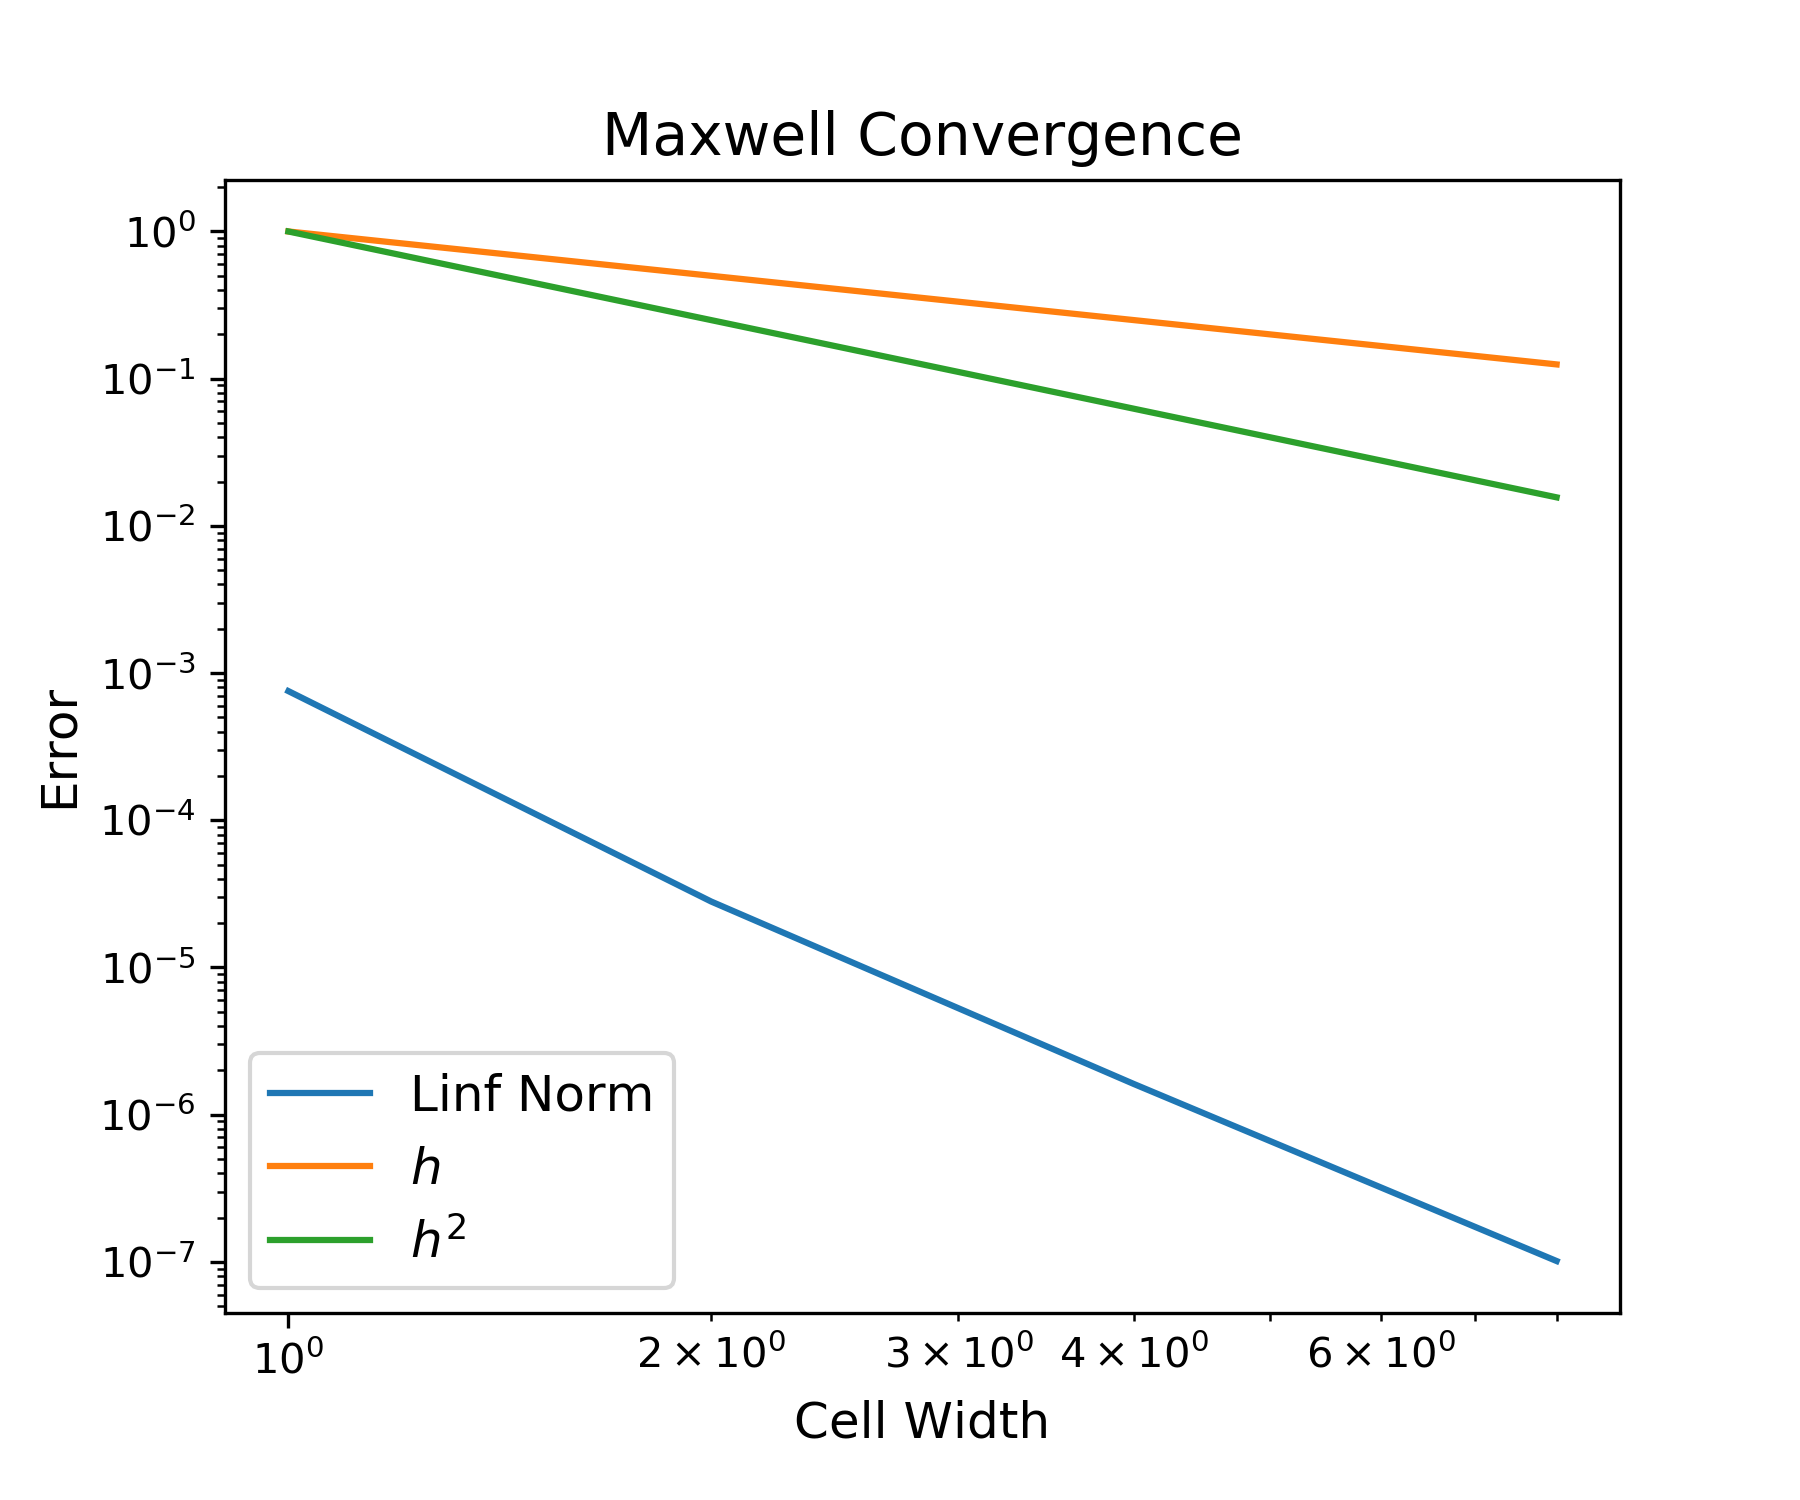
\includegraphics[scale=.6]{presentation/mx_conv.png}
                \end{center}

                Once again, very satisfying results, we see clear second order convergence in all three fields of our solution. One other note on this solver is that it is rather slow and the time step has to be fairly small in order for the solver to be stable. This is unexpected since we are using backward Euler so this probably indicates there is an issue somewhere in the code. 

            \section*{Incompressible Navier-Stokes}

            Our equations for incompressible Navier-Stokes are given by:
    \begin{align*}
        \rho \left(\frac{\partial \boldsymbol{u}}{\partial t} + \boldsymbol{u} \cdot \nabla \boldsymbol{u}\right) + \nabla p &= \mu \Delta \boldsymbol{u} + \boldsymbol{f}_L,\\
        -\nabla \cdot \boldsymbol{u} &= 0,
    \end{align*}
    where $\boldsymbol{f}_L$ is the Lorenz force defined using the magnetic field. Notice that if we use the method of manufactured solutions to solve this system, the Lorenz force becomes obsolete. So for this section, we will ignore the Lorenz force and replace $\boldsymbol{f}_L$ with $\boldsymbol{f}$.

    Once again we can look at the vector form of this system
    \[
        \begin{bmatrix} \rho \left(\frac{\partial \boldsymbol{u}}{\partial t} + \boldsymbol{u} \cdot \nabla \boldsymbol{u}\right) + \nabla p - \mu \Delta \boldsymbol{u} \\ -\nabla \cdot \boldsymbol{u} \end{bmatrix} = \begin{bmatrix} \boldsymbol{f} \\ 0 \end{bmatrix},
        \]
        which can be multiplied on the left by the test function $\phi = \begin{bmatrix}\boldsymbol{v} \\ w \end{bmatrix}$ to obtain the weak form:
            \[
        \rho\left(\boldsymbol{v},\frac{\partial \boldsymbol{u}}{\partial t} \right)_\Omega
        + \rho (\boldsymbol{v},\boldsymbol{u} \cdot \nabla \boldsymbol{u})_\Omega
        -\mu ( \boldsymbol{v}, \Delta \boldsymbol{u}) _\Omega 
        + ( \boldsymbol{v}, \nabla p) _\Omega
        - (w, \nabla \cdot \boldsymbol{u})_\Omega = (\boldsymbol{v},\boldsymbol{f})_\Omega.
    \]
    Once again we can apply integration by parts to the third and fourth terms on the left to obtain
        \[
        \rho\left(\boldsymbol{v},\frac{\partial \boldsymbol{u}}{\partial t} \right)_\Omega
        + \rho (\boldsymbol{v},\boldsymbol{u} \cdot \nabla \boldsymbol{u})_\Omega
        + \mu (\nabla \boldsymbol{v}, \nabla \boldsymbol{u}) _\Omega 
        - (\nabla \cdot \boldsymbol{v}, p) _\Omega
        - (w, \nabla \cdot \boldsymbol{u})_\Omega = (\boldsymbol{v},\boldsymbol{f})_\Omega.
    \]
    Now there are a few issues at play in this system. One is the nonlinearity in the second term on the left hand side. This nonlinearity can be addressed in a number of ways, including using an IMEX solver and handling the nonlinearity with the previous velocity values, using newton iterations instead of a linear solve, or approximating one of the velocity vectors involved in the nonlinear term. The other issue is the coupling of the pressure and the velocity. 

    In this system, the coupled pressure and velocity produce a very poor condition number. More specifically the issue occurs from the coupling of the diffusion operator and the incompressibility condition. If we chose to leave the two components coupled, we can try to resolve this discontinuity by using grad-div stabilitization. This amounts to adding the term $[\gamma \nabla (\nabla \cdot \boldsymbol{u})]$ to the conservation of momentum equation. Notice that because the velocity is divergence free, in the continuous case this does not affect the solution. After applying the grad-div stabilization, we can use a Schur decomposition to solve the system again. We must be much more cautious in choosing preconditioners for the block Schur system in this case since the condition number is much worse. 
   
   I attemped to solve this system with grad-div stabilization using an IMEX solver to resolve the nonlinearity without any luck. I tried a variety of different preconditioners from the literature \cite{gd1,gd2,gd3} but was unable to resolve the ill-conditioned system in the end.

   Since keeping the diffusion and incompressiblity condition coupled was unsuccessful, we now use a different method that decouples the two components to avoid the ill-conditioned matrix we encountered with the coupled system. For more resources on the motivation for projection methods for incompressible Navier-Stokes, see \cite{projection}. In this code, we use the projection method outlined in \cite{rotational}. 

   The projection method can be broken up into four steps. To start, assume that we have solutions for velocity and pressure at the first and second time step. 

   \begin{enumerate}
       \item First we extrapolate approximations of the velocity and pressure. The purpose of extrapolation the velocity is for computing the nonlinear term of the momentum equation. And the extrapolated pressure is also used for the lagging pressure term in the momentum equation. In both cases, we could simply use the velocity and pressure at the previous time step instead of doing this extrapolation. 
           \[
               \boldsymbol{u}^* = 2\boldsymbol{u}^k - \boldsymbol{u}^{k-1},\quad p^* = p^k + \frac{4}{3}\phi^k-\frac{1}{3}\phi^{k-1}, 
           \]
           where each $\phi^k$ is an auxillary function that arises when we take the projection specified by the solution of a Poisson equation (shown below).
       \item Next we handle the diffusion by solving the following system for an approximation of $\boldsymbol{u}^{k+1}$ given by $\tilde{\boldsymbol{u}}^{k+1}$ 
           \[
               \frac{1}{2\Delta t}(3\tilde{\boldsymbol{u}}^{k+1} - 4\boldsymbol{u}^k + \boldsymbol{u}^{k-1}) + \boldsymbol{u}^*\cdot \nabla \tilde{\boldsymbol{u}}^{k+1} + \frac{1}{2}(\nabla \cdot \boldsymbol{u}^*)\tilde{\boldsymbol{u}}^{k+1} -\mu \Delta \tilde{\boldsymbol{u}}^{k+1} + \nabla p^* = \boldsymbol{f}^{k+1}.
           \]
           Note that the advection term has been replaced by the skew-symmetric version which will not make a difference in the true solution as a result of the incompressibility condition. Using this form helps ensure stability of the time discretization. 
       \item Now we will formulate the projection by considering the above equation with the true solution $\boldsymbol{u}^{k+1}$ which satisfies the divergence-free condition, and the true pressure solution $p^{k+1}$. Ignoring the nonlinear terms, we can subtract this "correct" system from the approximated one to obtain the following
           \[
               \frac{3}{2\Delta t}(\tilde{\boldsymbol{u}}^{k+1} - \boldsymbol{u}^{k+1}) -\mu \Delta (\tilde{\boldsymbol{u}}^{k+1} - \boldsymbol{u}^{k+1}) + \nabla (p^* - p^{k+1}) = 0.
           \]
           Now we can take the divergence of this equation and apply the incompressibility condition on $\boldsymbol{u}^{k+1}$ to obtain
           \[
               \frac{3}{2\Delta t}\nabla \cdot \tilde{\boldsymbol{u}}^{k+1} = \Delta (p^{k+1} - p^* + \mu \nabla \cdot \tilde{\boldsymbol{u}}^{k+1}).
           \]
           At this point we define our auxillary variable
           \[
               \phi^{k+1} = p^{k+1} - p^k +\mu \nabla \cdot \tilde{\boldsymbol{u}}^{k+1},
           \]
           notice we use the previous pressure solution instead of the extrapolated pressure value. So at this point we solve the following for $\phi^{k+1}$
           \[
               \Delta \phi^{k+1} = \frac{3}{2\Delta t}\nabla \cdot \tilde{\boldsymbol{u}}^{k+1} ,
           \]
           with $\phi^{k+1}$ having zero Neumann boundary conditions on the domain boundary. More details on these boundary conditions can be found in \cite{timmerman}.
       \item Finally we solve for the updated pressure given by
           \[
               p^{k+1} = p^k + \phi^{k+1} - \mu \nabla \cdot \tilde{\boldsymbol{u}}^{k+1}.
           \]
           In most projection-correction schemes the pressure update is first order, but with the extra divergence subtracted off, this scheme is referred to as a rotational projection-correction scheme and the pressure update should be second order \cite{rotational}.
   \end{enumerate}

   \subsection*{Testing the Navier-Stokes Solver}

            To test the convergence of this solver, I used the following exact solution,
            \[ \begin{bmatrix} \boldsymbol{h} \\ q\end{bmatrix} = \begin{bmatrix} t \cos(y) \\ t \sin(y) \\ txy \end{bmatrix}.\]
                The approximated solution for the velocity field in the $x$-component is shown in the figure below.

                \begin{center}
                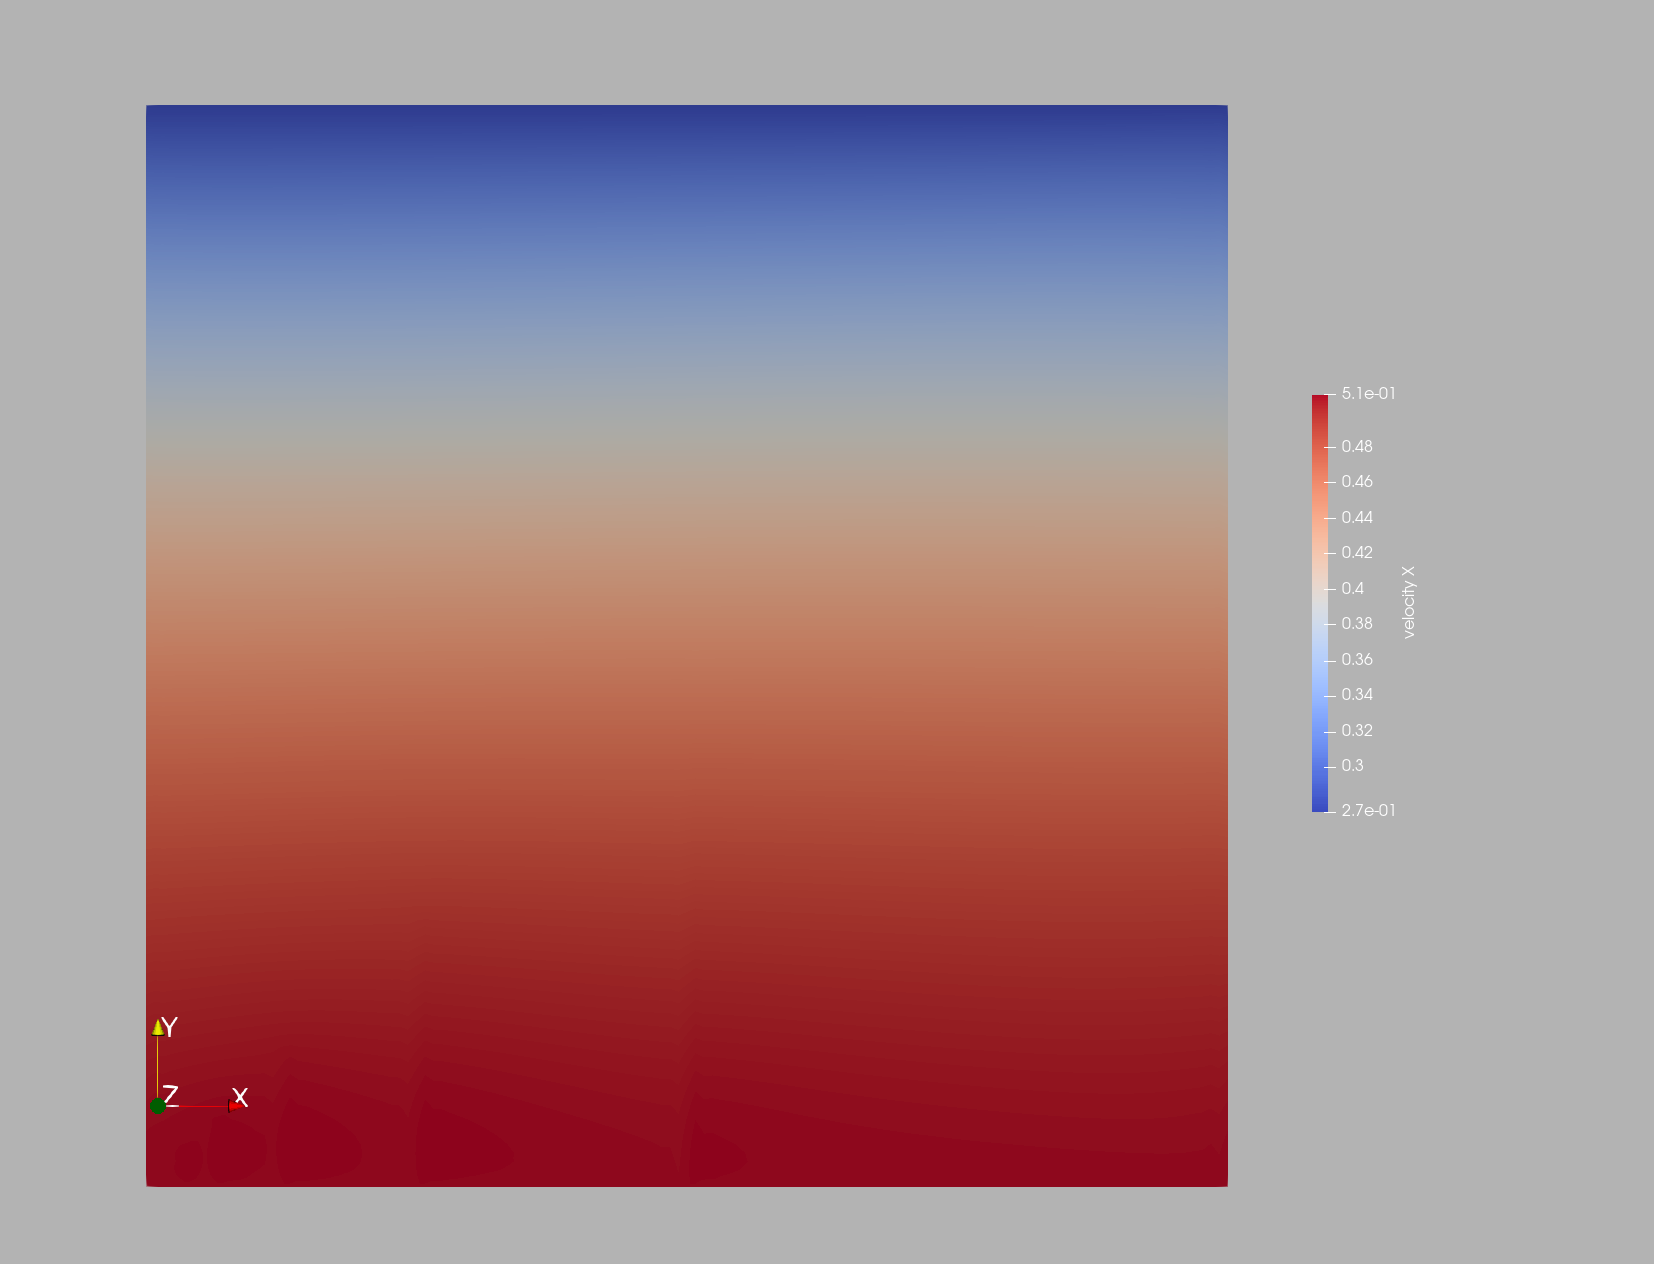
\includegraphics[scale=.2]{vel_x.png}
                \end{center}

                And the velocity field in the $y$-component:

                \begin{center}
                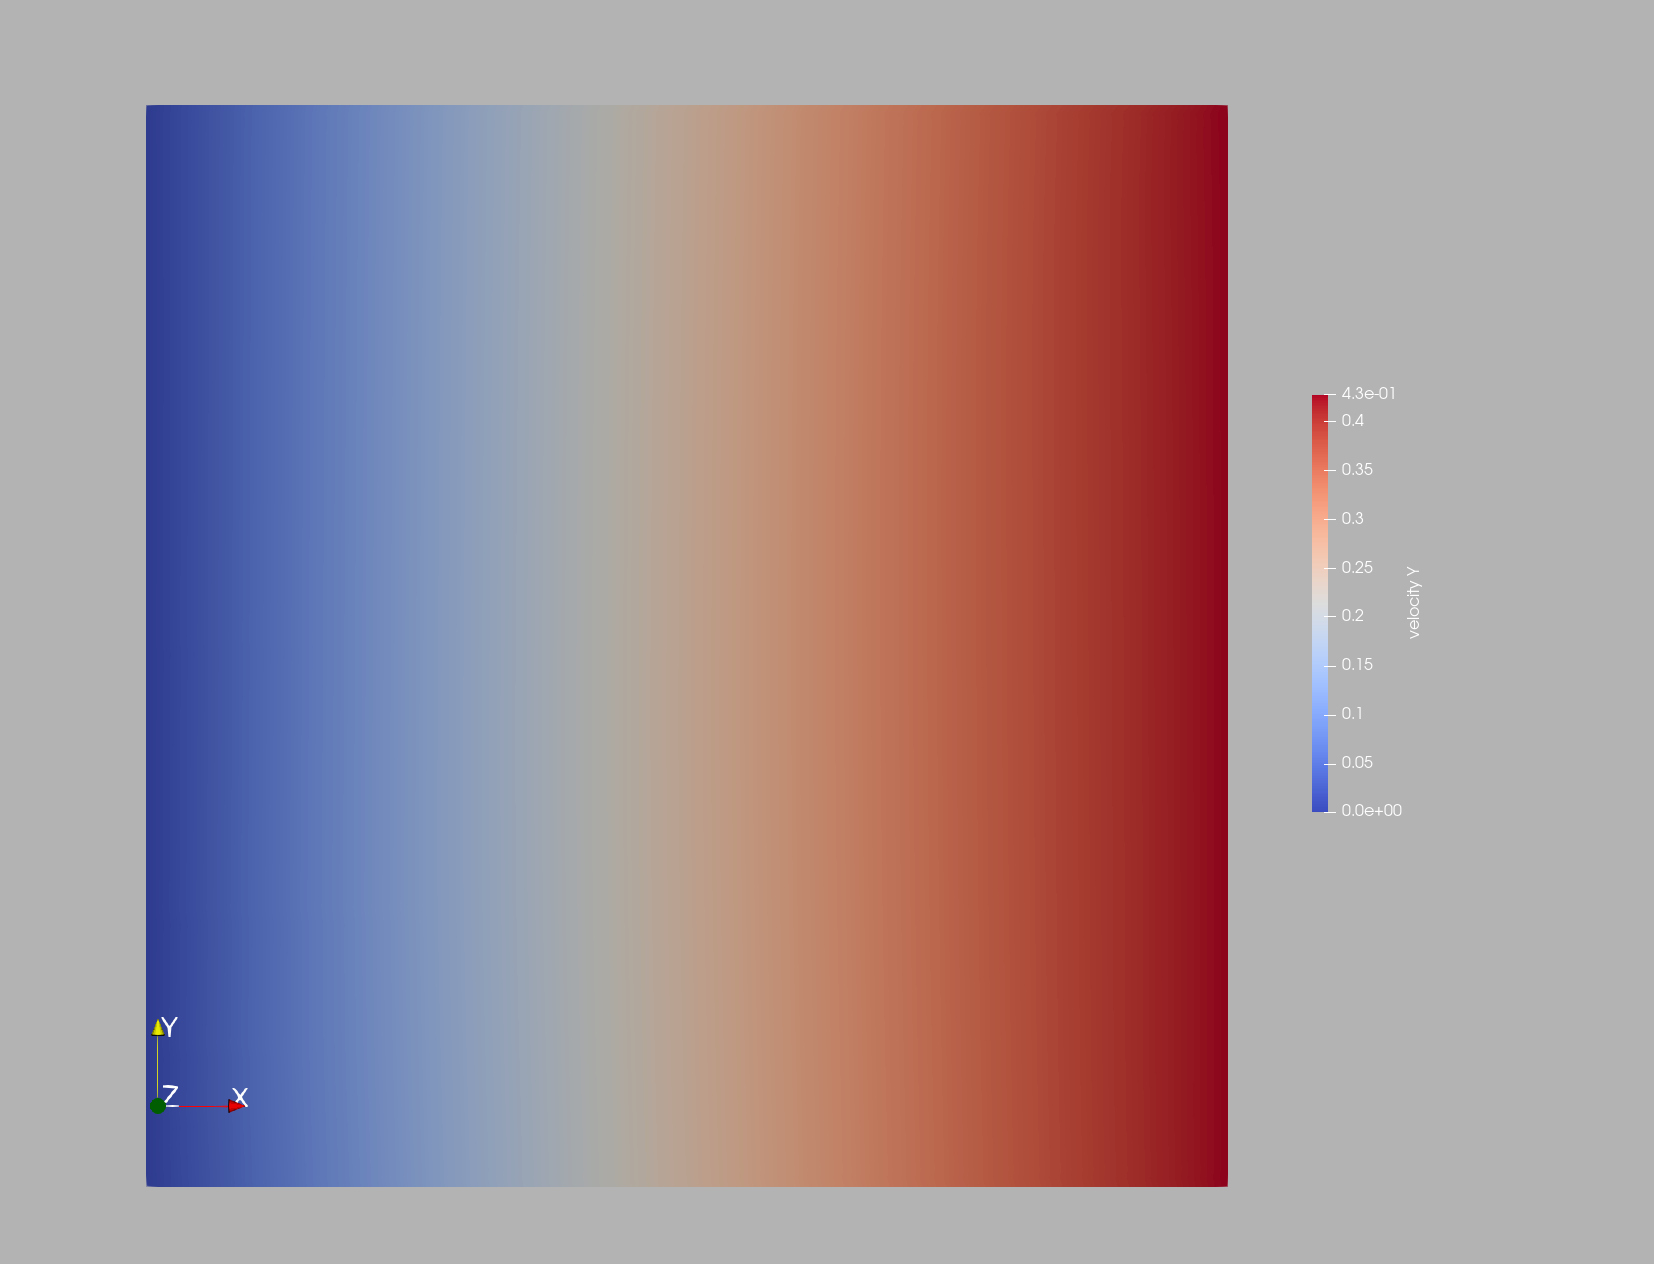
\includegraphics[scale=.2]{vel_y.png}
                \end{center}

                Finally, the solution to the pressure field is shown below. In this solution we see a very strange behavior that is not expected. I will mention this more below.

                \begin{center}
                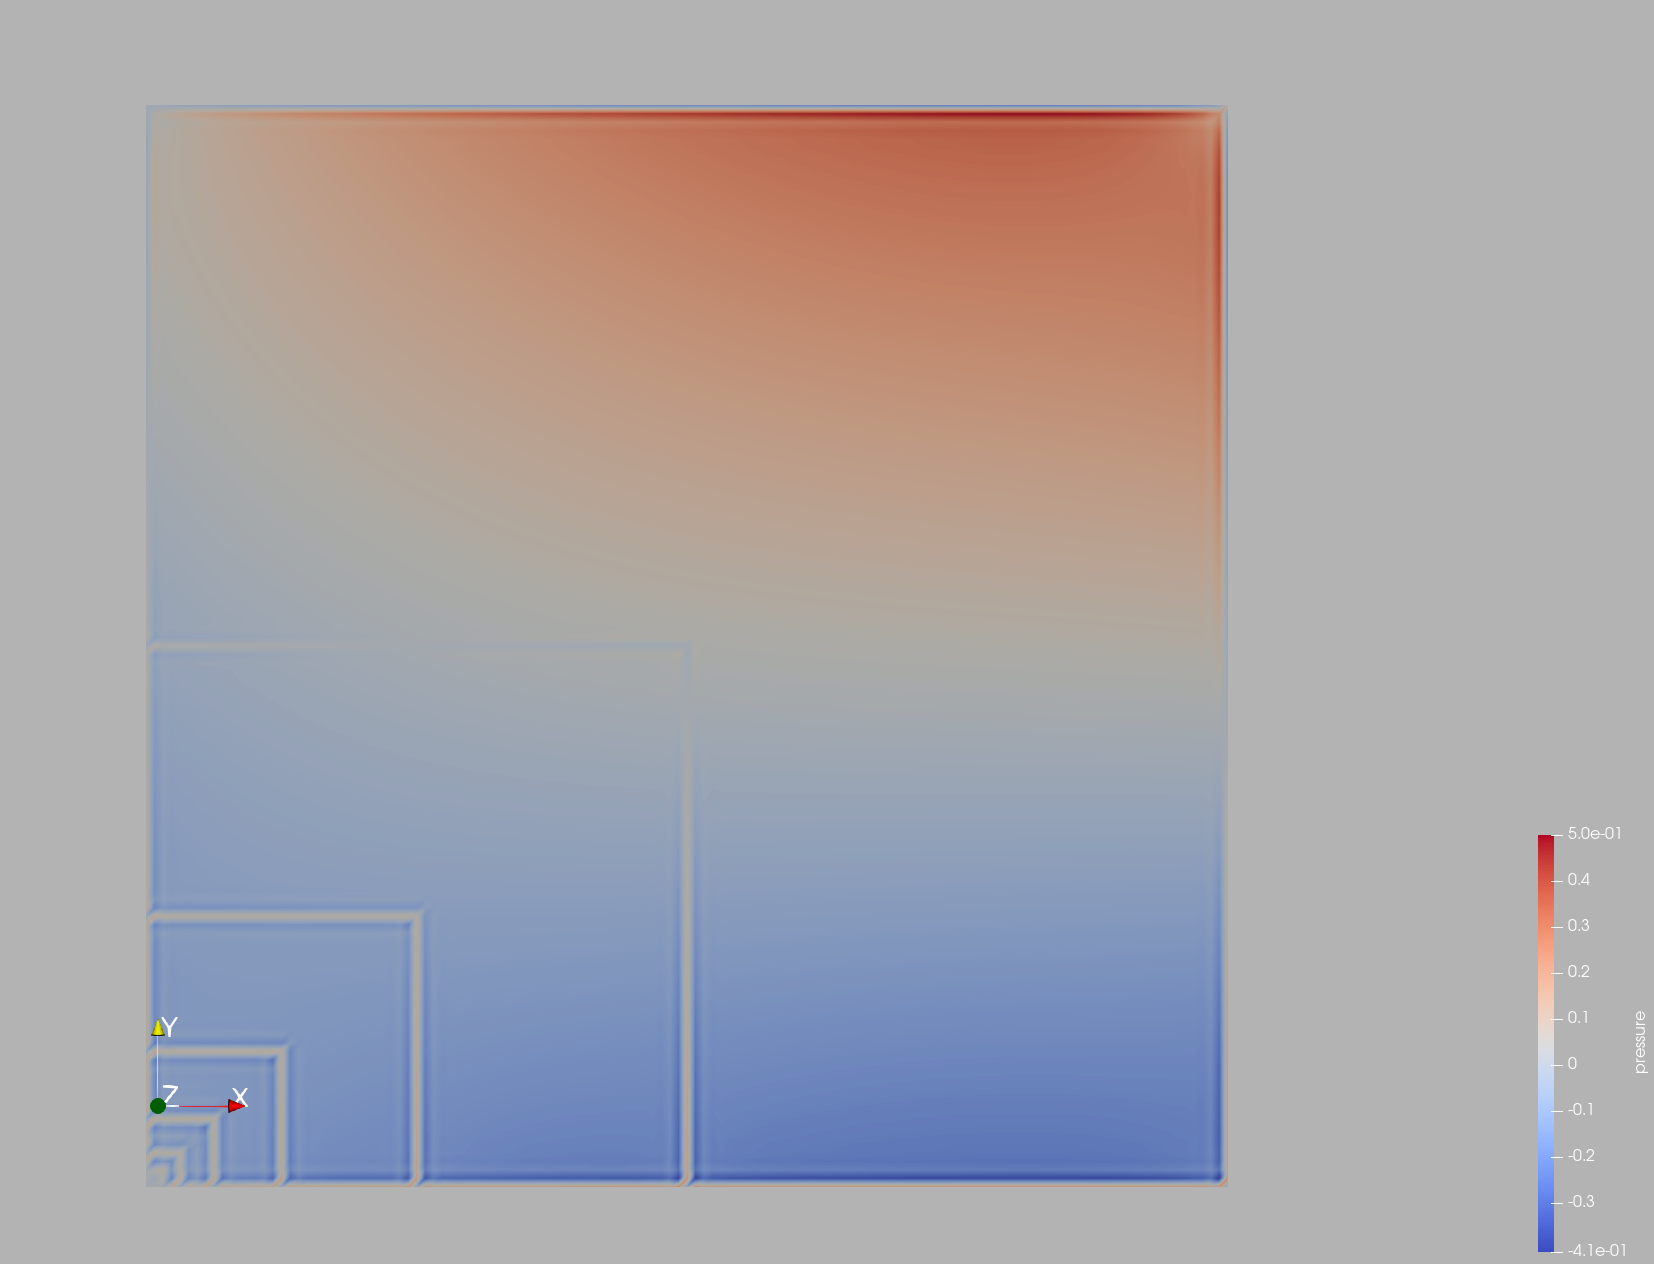
\includegraphics[scale=.2]{pressure.png}
                \end{center}

                In this case, the velocity results look fairly good while the pressure is not ideal. The following graph shows the convergence results for the velocity and pressure separately. Recall that with our rotational projection formulation, we expect second order accuracy in the pressure update as opposed to first. However, in the graph below we see that while we are getting roughly second order accuracy in the velocity, we only have first order accuracy in the pressure. 

                From this is appears that there is likely an issue in how the method was implemented that accounts for the strange behavior visible in the pressure solution as well as the poor convergence rate. One thing to note is that with standard projection methods, there is a non-physical boundary condition imposed on the pressure update that usually causes convergence issues, however, this is supposed to be resolved with the rotational form that I used. But we see the maximum error occuring on the top boundary of the domain so it could be that there is some issue happening with the boundary conditions.

                \begin{center}
                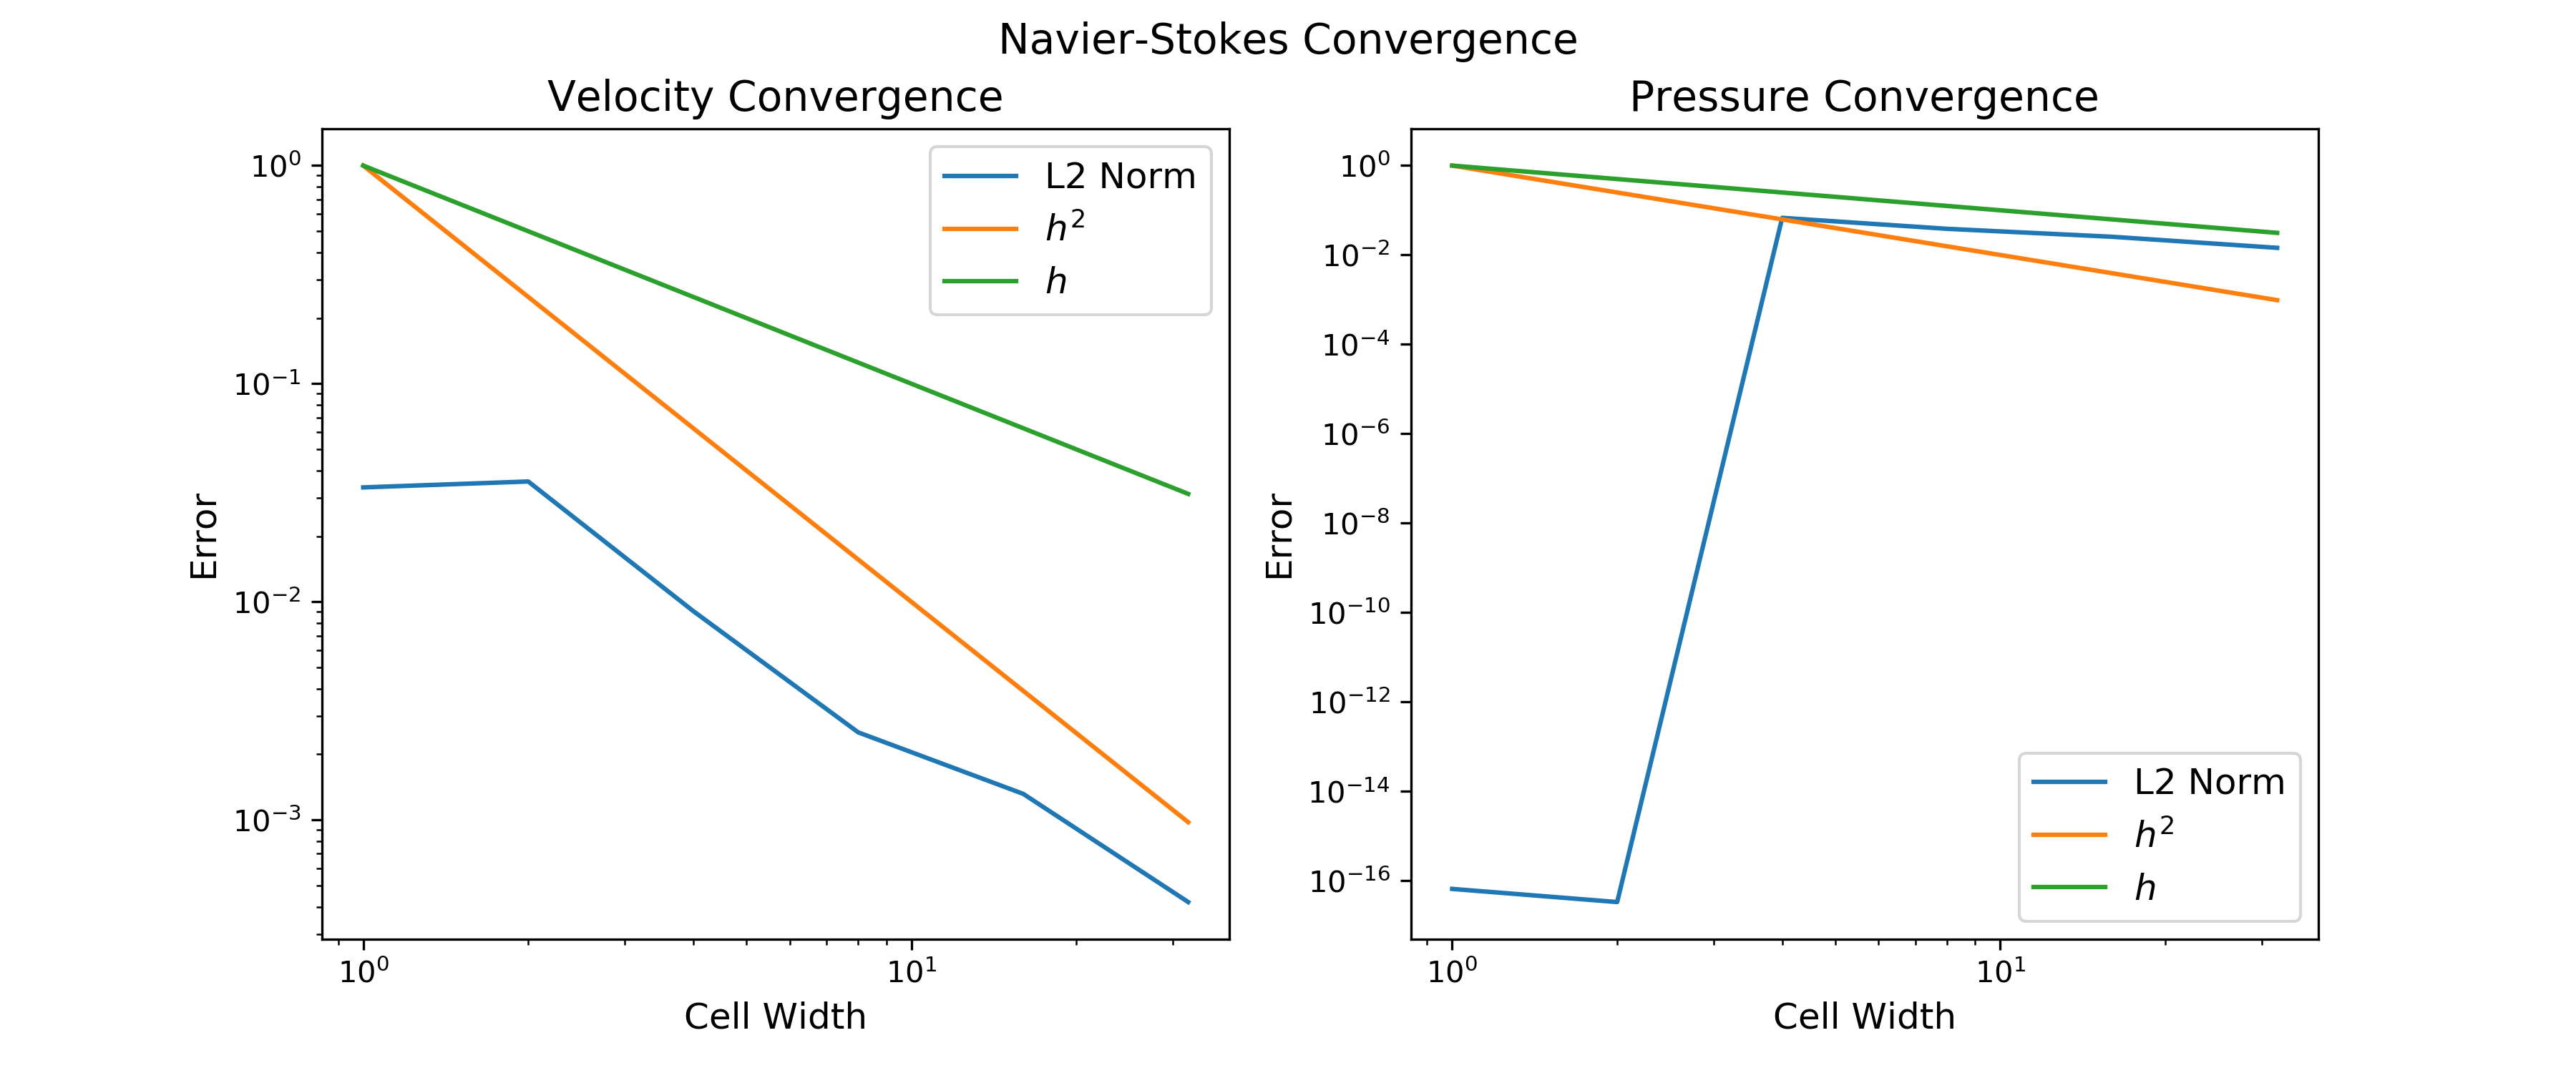
\includegraphics[scale=.6]{presentation/ns_conv.png}
                \end{center}

   \section*{Coupled MHD}

   Now that we have outlined solvers for both the Maxwell's sytem and the Navier-Stokes equations, we are prepared to couple the two together. To do this we will first initialize all our parameters with the given initial conditions. Then we will start by solving the Maxwell's equations to update the magnetic field. And with the updated magnetic field we will then solve incompressible Navier-Stokes to update the pressure and velocity. 

   Since the projection method starts after an initial time and an additional time have been computed, we will iterate the Maxwell solver twice before we begin also solving the Navier-Stokes equations so that the magnetic field does not lag one step behind the velocity and pressure. 

   Unfortunately we can not use the method of manufactured solutions to test our coupled solver since the coupling occurs in the forcing function of the Navier-Stokes equations, so instead we will need exact solutions to test the accuracy of our solver. At the present time we will test the code on a simple constant solution which will give insight into if our coupled solver is set up correctly and is functioning somewhat as we expect. 


   \subsection*{Testing the Coupled Solver}

   As mentioned, we will test the solver on just a constant exact solution. Unfortunately the coupled solver does very poorly, much worse than both methods separately with a constant field. This does not make sense to me because with a constant field they should bold be solving the system exactly or almost exactly so there must be an bug in the code that came up when the two solvers were combined into one file. However, at this point I have spent so long trying to get a second order Navier-Stokes solver working without any luck and I am not extremely motivated to get the coupled solver working right now since it will need to be modified once I figure a more accurate fluid solve. So there is little reason to put too much time into this one currently. 

   The poor convergence results are shown in the figure below. 

                \begin{center}
                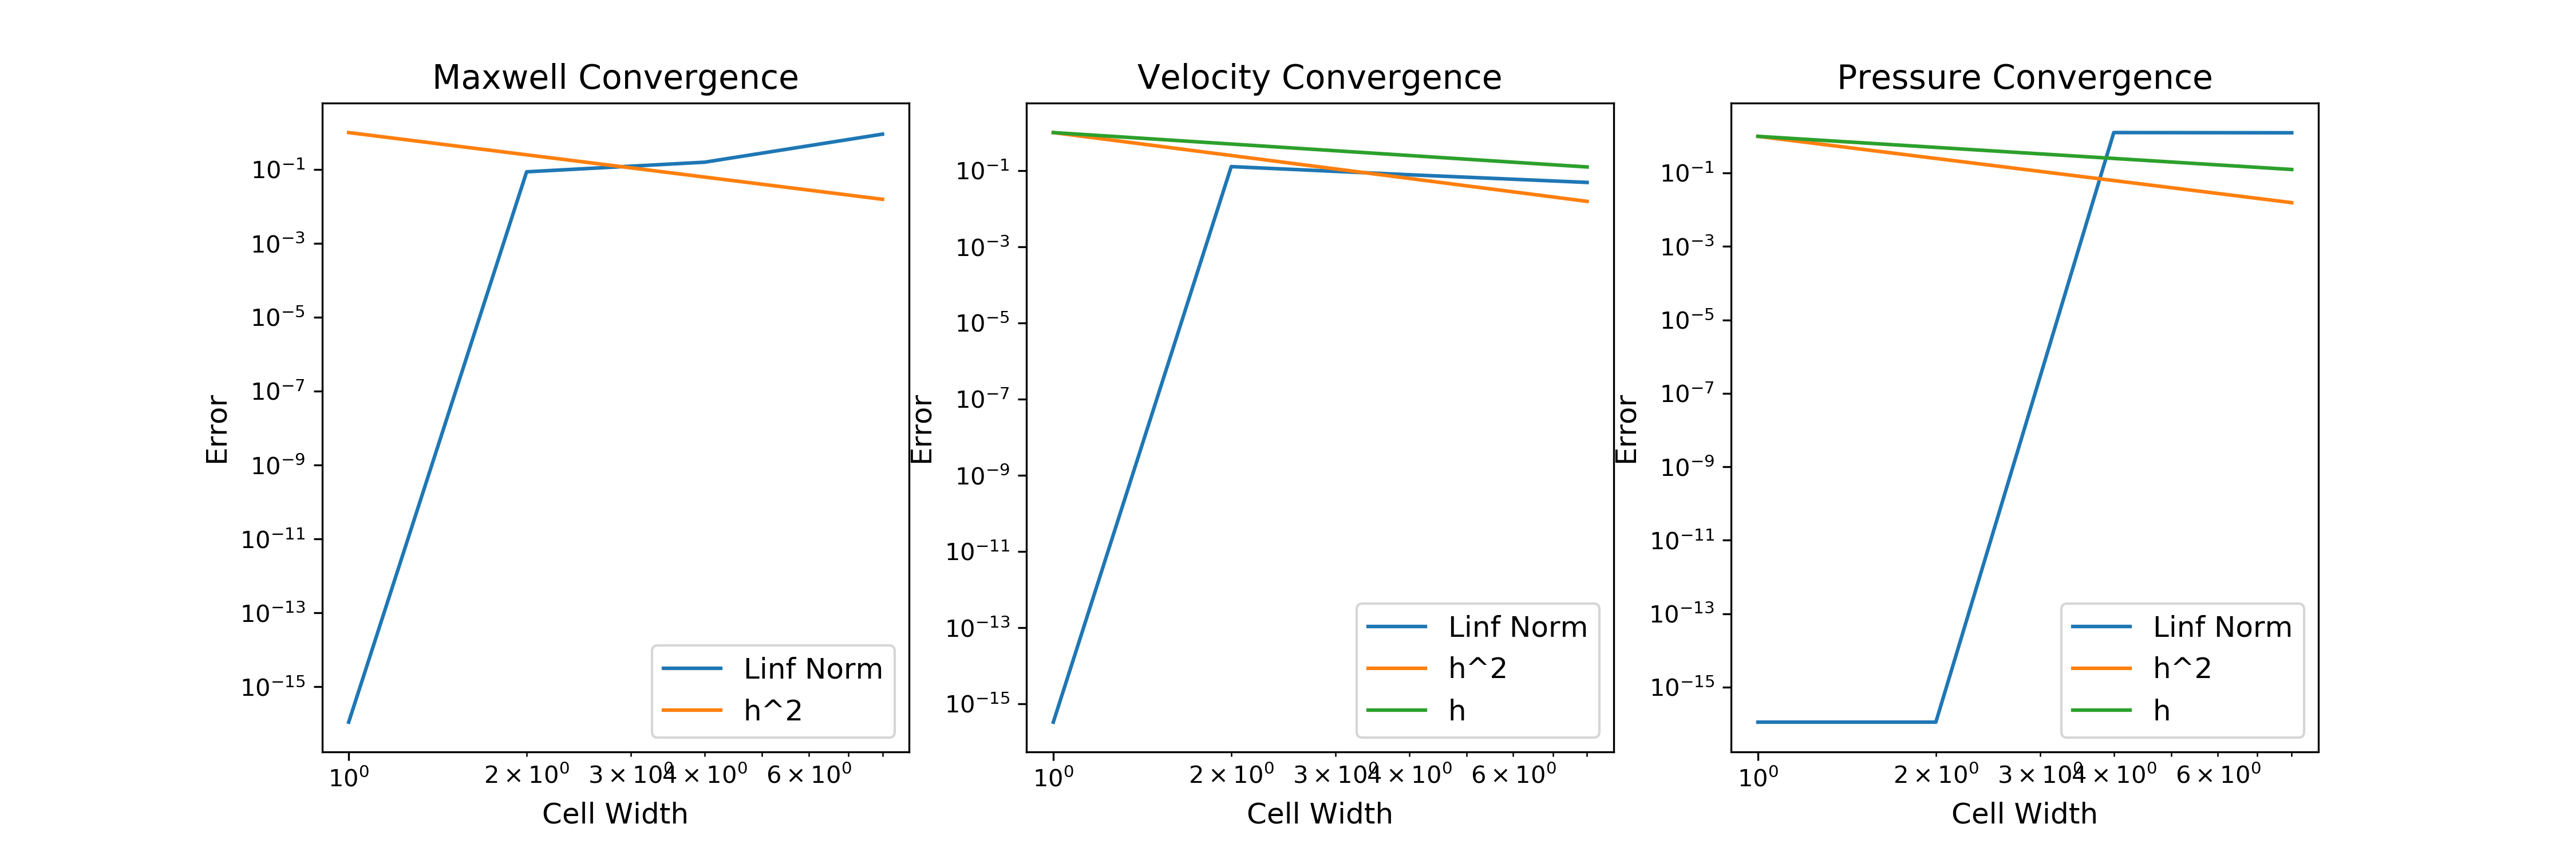
\includegraphics[scale=.4]{presentation/full_conv.png}
                \end{center}


   \section*{The Code}

   \subsection*{Include files}
   Including all the necessary files for both solvers. 
   \begin{lstlisting}
   #include <deal.II/base/convergence_table.h>
#include <deal.II/base/function.h>
#include <deal.II/base/quadrature_lib.h>
#include <deal.II/base/utilities.h>

#include <deal.II/dofs/dof_accessor.h>
#include <deal.II/dofs/dof_handler.h>
#include <deal.II/dofs/dof_tools.h>
#include <deal.II/dofs/dof_renumbering.h>

#include <deal.II/fe/fe_q.h>
#include <deal.II/fe/fe_system.h>
#include <deal.II/fe/fe_nedelec_sz.h>
#include <deal.II/fe/fe_values.h>

#include <deal.II/grid/grid_generator.h>
#include <deal.II/grid/grid_tools.h>
#include <deal.II/grid/grid_out.h>
#include <deal.II/grid/grid_refinement.h>
#include <deal.II/grid/manifold_lib.h>
#include <deal.II/grid/tria.h>
#include <deal.II/grid/tria_accessor.h>
#include <deal.II/grid/tria_iterator.h>

#include <deal.II/lac/block_linear_operator.h>
#include <deal.II/lac/block_vector.h>
#include <deal.II/lac/block_sparse_matrix.h>
#include <deal.II/lac/affine_constraints.h>
#include <deal.II/lac/constrained_linear_operator.h>
#include <deal.II/lac/dynamic_sparsity_pattern.h>
#include <deal.II/lac/full_matrix.h>
#include <deal.II/lac/precondition.h>
#include <deal.II/lac/solver_gmres.h>
#include <deal.II/lac/sparse_direct.h>
#include <deal.II/lac/sparse_ilu.h>
#include <deal.II/lac/sparse_matrix.h>
#include <deal.II/lac/vector.h>

#include <deal.II/numerics/data_out.h>
#include <deal.II/numerics/error_estimator.h>
#include <deal.II/numerics/matrix_tools.h>
#include <deal.II/numerics/vector_tools.h>

#include <iostream>
#include <fstream>
#include <cmath>

\end{lstlisting}

I am using namespace dealii mainly because it makes coding much simpler.
\begin{lstlisting}
using namespace dealii;
\end{lstlisting}

\subsection*{Inverse Matrix Class}
This class is used twice in the Maxwell solver. It essentially computes the inverse of a matrix by solving with GMRES using a provided preconditioner. This is done by defining the vmult operation to solve the linear system.

\begin{lstlisting}
// Inverse Matrix Class used for creating the pressure mass matrix
// preconditioner (for the outer solve) and used to define the inverse
// of the Schur complement -- both for the Maxwell solver
template<class MatrixType, class PreconditionerType>
class InverseMatrix : public Subscriptor
{
    public:
        InverseMatrix(const MatrixType & m,
                      const PreconditionerType &p)
            : matrix(&m)
            , preconditioner(&p)
        {}

        void vmult(Vector<double> &sol, const Vector<double> &vec) const
        {
            SolverControl solver_control(vec.size(), 1e-6*vec.l2_norm());
            SolverGMRES<Vector<double>> gmres(solver_control);
            sol = 0;
            gmres.solve(*matrix, sol, vec, *preconditioner);
        }

    private:
        const SmartPointer<const MatrixType> matrix;
        const SmartPointer<const PreconditionerType> preconditioner;
};
\end{lstlisting}

\subsection*{Schur Complement Class}
This class simply defines the Schur complement of a system. Matrix-matrix multiplication is much more expensive than matrix-vector multiplication so this class defines a vmult operation that multiplies the three matrices that form the Schur complement by the given vector in order so as to avoid all matrix-matrix multiplication.
\begin{lstlisting}
// Defines the Schur complement given the block system and the A inverse
// used in Maxwell Solver
template<class InverseType>
class SchurComplement : public Subscriptor
{
    public:
        SchurComplement(const BlockSparseMatrix<double> &system_matrix,
                        const InverseType &A_inv)
            : system_matrix(&system_matrix)
            , A_inv(&A_inv)
            , tmp1(system_matrix.block(0,0).m())
            , tmp2(system_matrix.block(0,0).m())
        {}

        void vmult(Vector<double> &sol, const Vector<double> &vec) const
        {
            system_matrix->block(0,1).vmult(tmp1, vec);
            A_inv->vmult(tmp2, tmp1);
            system_matrix->block(1,0).vmult(sol, tmp2);
        }

    private:
        const SmartPointer<const BlockSparseMatrix<double> > system_matrix;
        const SmartPointer<const InverseType> A_inv;

        mutable Vector<double> tmp1, tmp2;
};
\end{lstlisting}

\subsection*{Exact Solutions}
Here we just define the exact solutions for all the fields in our system. The exact solutions for the magnetic field and its lagrange multiplier are stored together since the Maxwell solver stores these two components in one large system. Because we have decoupled the Navier-Stokes solver, we will be keeping the velocity and pressure functions separate and thus they have separate exact solutions. 

\begin{lstlisting}
// Exact solution for the magnetic field and
// for the lagrange multiplier in maxwell system
template<int dim>
class ExactMaxwell : public Function<dim>
{
    public:
        ExactMaxwell()
            : Function<dim>(dim+1) // 3
        {}

        virtual void
        vector_value(const Point<dim> &p,
                     Vector<double> &  values) const override
        {
            //const double time = this->get_time();
            (void)p;
            values(0) = 1.0;//time*cos(p(1));
            values(1) = 1.0;//time*sin(p(0));
            values(2) = 0;
        }
};

// Exact solution for velocity
template<int dim>
class ExactVelocity : public Function<dim>
{
    public:
        ExactVelocity()
            : Function<dim>(dim) // 3
        {}

        virtual void
        vector_value(const Point<dim> &p,
                     Vector<double> &  values) const override
        {
            //const double time = this->get_time();
            (void)p;
            values(0) = 1.0;
            values(1) = 1.0;
        }
};

// Exact solution for pressure
template<int dim>
class ExactPressure : public Function<dim>
{
    public:
        ExactPressure()
            : Function<dim>(1) // 3
        {}

        virtual
        double value(const Point<dim> &p,
                     unsigned int component = 0) const override
        {
            (void)p;
            (void)component;
            //const double time = this->get_time();
            return 1.0;
        }
};
\end{lstlisting}

\subsection*{MHD Solver Class}
Here we have the main definiton and constructor of the MHD solver class. The functions will be discussed later in the code but there are a few things to mention. One is that the Maxwell solver stores a constrained and unconstrained system matrix and mass matrix which was done so that only the right hand side would need to be recomputed each time step. However when coupled with Navier-Stokes, the left hand side now also needs to be recomputed with each time step so this is somewhat redundant and could be replaced. Also notice that as mentioned, we have separate dof\_handlers and constraints for the velocity and pressure even though they are both in the Navier-Stokes system.

\begin{lstlisting}
// Main class for MHD solver
template <int dim>
class MHD
{
    public:
        MHD(const unsigned int degree,
            const unsigned int n_global_refinements);

        void run();

    private:
        void setup_grid();
        void output_results();

        // maxwell functions
        void setup_maxwell_dofs();
        void assemble_maxwell_system(bool initial);
        void solve_maxwell(bool update);

        // navier stokes functions
        void setup_ns_dofs();
        void assemble_ns_matrices();
        void initialize_ns_system();
        void assemble_lorenz_force();
        void ns_diffusion_step();
        void ns_projection_step();
        void ns_pressure_step();
        void assemble_ns_advection_matrix();
        void solve_ns();

        const unsigned int degree;
        unsigned int n_global_refinements;

        // time stepping
        double time_step;
        double end_time;
        double current_time;
        int    time_step_number;

        // parameters
        double nu;
        double beta;
        double eta;
        double mu;
        double rho;

        // which pressure update
        bool standard;

        Triangulation<dim> triangulation;

        // finite elements
        FESystem<dim>      fe_maxwell;
        FESystem<dim>      fe_velocity;
        FE_Q<dim>          fe_pressure;

        // dof handlers
        DoFHandler<dim>    maxwell_dof_handler;
        DoFHandler<dim>    velocity_dof_handler;
        DoFHandler<dim>    pressure_dof_handler;

        // constraints
        AffineConstraints<double> maxwell_constraints;
        AffineConstraints<double> velocity_constraints;
        AffineConstraints<double> pressure_constraints;

        // matrices for maxwell solver
        BlockSparsityPattern      maxwell_sparsity_pattern;
        BlockSparsityPattern      maxwell_unconstrained_sparsity_pattern;
        BlockSparseMatrix<double> maxwell_system_matrix;

        BlockSparseMatrix<double> maxwell_unconstrained_system_matrix;
        BlockSparseMatrix<double> maxwell_unconstrained_mass_matrix;

        BlockSparsityPattern      maxwell_preconditioner_sparsity_pattern;
        BlockSparseMatrix<double> maxwell_preconditioner_matrix;
        SparseMatrix<double>      maxwell_lagrange_mass_matrix;

        // vectors for maxwell solver
        BlockVector<double> current_maxwell;
        BlockVector<double> previous_maxwell;
        BlockVector<double> maxwell_system_rhs;
        BlockVector<double> maxwell_load_vector;

        // matrices for ns solver
        SparsityPattern      velocity_sparsity_pattern;
        SparsityPattern      pressure_sparsity_pattern;
        SparsityPattern      vel_pres_sparsity_pattern;

        SparseMatrix<double> velocity_laplace_matrix;
        SparseMatrix<double> pressure_laplace_matrix;

        SparseMatrix<double> velocity_mass_matrix;
        SparseMatrix<double> pressure_mass_matrix;

        SparseMatrix<double> advection_matrix;
        SparseMatrix<double> gradient_matrix;

        SparseMatrix<double> velocity_step_matrix_const;
        SparseMatrix<double> velocity_step_matrix;
        SparseMatrix<double> pressure_step_matrix;

        // vectors for ns solver
        Vector<double> lorenz_force;
        Vector<double> diffusion_rhs;
        Vector<double> projection_rhs;

        Vector<double> previous_velocity;
        Vector<double> current_velocity;
        Vector<double> previous_pressure;
        Vector<double> current_pressure;
        Vector<double> previous_phi;
        Vector<double> current_phi;

        Vector<double> u_star;
        Vector<double> p_star;

        // preconditioners for ns solver
        SparseDirectUMFPACK pressure_mass_inv;
        SparseDirectUMFPACK pressure_laplace_inv;
        SparseILU<double>   diffusion_preconditioner;
        SparseILU<double>   projection_preconditioner;

        // exact solutions (used for BCs too)
        ExactMaxwell<dim>   exact_maxwell;
        ExactVelocity<dim> exact_velocity;
        ExactPressure<dim> exact_pressure;

};

// MHD constructor
template <int dim>
MHD<dim>::MHD(const unsigned int degree,
              const unsigned int n_global_refinements)
    : degree(degree)
    , n_global_refinements(n_global_refinements)
    , time_step(std::pow(0.1, n_global_refinements))
    , end_time(1.0)
    , current_time(0.0)
    , time_step_number(1)
    , nu(1.0)
    , beta(1.0)
    , eta(0.1)
    , mu(1.0)
    , rho(1.0)
    , standard(false)
    , fe_maxwell(FE_NedelecSZ<dim>(degree+1), 1, FE_Q<dim>(degree), 1)
    , fe_velocity(FE_Q<dim>(degree+1), dim)
    , fe_pressure(degree)
    , maxwell_dof_handler(triangulation)
    , velocity_dof_handler(triangulation)
    , pressure_dof_handler(triangulation)
{}
\end{lstlisting}

\subsection*{Setting up the Grid}
For this solver we use a regular 2D hyper cube with increasing refinement levels in order to see convergence rates. 
\begin{lstlisting}
// set up the grid - basic hyper cube with specified refinement
template <int dim>
void
MHD<dim>::setup_grid()
{
  GridGenerator::hyper_cube(triangulation);

  triangulation.refine_global(n_global_refinements);

  // maxwell can't handle faster time stepping but ns can
  //double dx = GridTools::minimal_cell_diameter(triangulation);
  // time_step = dx; // this will just speed things up
}
\end{lstlisting}

\subsection*{Setting up the degrees of freedom}
We first setup the degrees of freedom for the Maxwell system. This is slightly more complicated than it is for the Navier-Stokes system because we are solving for the magnetic field and lagrange multiplier together. We want to have a block system so we need to sort the degrees of freedom by component.

\begin{lstlisting}
// setup dofs for maxwell system
// separate magnetic and lagrange components
// to ensure system has block structure
template <int dim>
void MHD<dim>::setup_maxwell_dofs()
{
    // make sure system is clear
    maxwell_system_matrix.clear();
    maxwell_unconstrained_mass_matrix.clear();
    maxwell_unconstrained_system_matrix.clear();
    maxwell_preconditioner_matrix.clear();
    maxwell_lagrange_mass_matrix.clear();

    maxwell_dof_handler.distribute_dofs(fe_maxwell);
\end{lstlisting}
Here is where we group the magentic field components separately from the lagrange multiplier components.
\begin{lstlisting}
    // group together the magentic field components
    // separate from the lagrange multiplier
    std::vector<unsigned int> block_component(dim + 1, 0);
    block_component[dim] = 1;

    DoFRenumbering::component_wise(maxwell_dof_handler);

    std::vector<types::global_dof_index> dofs_per_component(
            dim+1, types::global_dof_index(0));

    DoFTools::count_dofs_per_component(maxwell_dof_handler,
                                       dofs_per_component,
               true); // this means there will be no dublicates

    const unsigned int n_h = dofs_per_component[0];
    const unsigned int n_q = dofs_per_component[dim];
\end{lstlisting}
Now we will build the boundary conditions into the constraints. Because we update the boundary conditions at each time step and we really only care about structure right now, we could use zero functions to initialize the constraints instead of the exact solution. 

Since we are using Nedelec elements for the magnetic field, we cannot use the standard boundary value interplator, instead we use one designed specifically for the Nedelec element. And for the Lagrange multiplier we use the standard.
\begin{lstlisting}
    // it is overkill to use exact solution here
    exact_maxwell.set_time(current_time);

    {
      maxwell_constraints.clear();
      DoFTools::make_hanging_node_constraints(maxwell_dof_handler,
                                              maxwell_constraints);

      // FE_Nedelec boundary condition.
      VectorTools::project_boundary_values_curl_conforming_l2(
          maxwell_dof_handler,
          0,
          exact_maxwell,
          0,
          maxwell_constraints,
          StaticMappingQ1<dim>::mapping);

      FEValuesExtractors::Scalar q(dim);

      // Lagrange multiplier boundary conditions
      VectorTools::interpolate_boundary_values(maxwell_dof_handler,
                                               0,
                                               exact_maxwell,
                                               maxwell_constraints,
                                               fe_maxwell.component_mask(q));
    }
    maxwell_constraints.close();
    \end{lstlisting}
Now we are ready to define our sparsity patterns and initalize all the system's matrices and vectors based on the sparsity patterns. We setup three separate sparsity patterns here for the system, the unconstrained system, and the preconditioners. 
\begin{lstlisting}
    // setup sparsity patterns using constraints
    {
        BlockDynamicSparsityPattern dsp(2, 2);
        dsp.block(0, 0).reinit(n_h, n_h);
        dsp.block(1, 0).reinit(n_q, n_h);
        dsp.block(0, 1).reinit(n_h, n_q);
        dsp.block(1, 1).reinit(n_q, n_q);

        dsp.collect_sizes();

        Table<2, DoFTools::Coupling> coupling(dim + 1, dim + 1);

        DoFTools::make_sparsity_pattern(
          maxwell_dof_handler, dsp, maxwell_constraints, false);

        maxwell_sparsity_pattern.copy_from(dsp);
    }

    {
        BlockDynamicSparsityPattern unconstrained_dsp(2, 2);
        unconstrained_dsp.block(0, 0).reinit(n_h, n_h);
        unconstrained_dsp.block(1, 0).reinit(n_q, n_h);
        unconstrained_dsp.block(0, 1).reinit(n_h, n_q);
        unconstrained_dsp.block(1, 1).reinit(n_q, n_q);

        unconstrained_dsp.collect_sizes();

        DoFTools::make_sparsity_pattern(maxwell_dof_handler,
                                        unconstrained_dsp);
        maxwell_unconstrained_sparsity_pattern.copy_from(unconstrained_dsp);
    }


    {
        BlockDynamicSparsityPattern preconditioner_dsp(2, 2);
        preconditioner_dsp.block(0, 0).reinit(n_h, n_h);
        preconditioner_dsp.block(1, 0).reinit(n_q, n_h);
        preconditioner_dsp.block(0, 1).reinit(n_h, n_q);
        preconditioner_dsp.block(1, 1).reinit(n_q, n_q);

        preconditioner_dsp.collect_sizes();

        DoFTools::make_sparsity_pattern(maxwell_dof_handler,
                                      preconditioner_dsp,
                                      maxwell_constraints,
                                      false);

        maxwell_preconditioner_sparsity_pattern.copy_from(preconditioner_dsp);
    }

    // initialize matrices with sparsity patterns
    maxwell_system_matrix.reinit(maxwell_sparsity_pattern);
    maxwell_preconditioner_matrix.reinit(
            maxwell_preconditioner_sparsity_pattern);
    maxwell_lagrange_mass_matrix.reinit(
            maxwell_preconditioner_sparsity_pattern.block(1,1));
    maxwell_unconstrained_mass_matrix.reinit(
            maxwell_unconstrained_sparsity_pattern);
    maxwell_unconstrained_system_matrix.reinit(
            maxwell_unconstrained_sparsity_pattern);

    // initialize vectors with sparsity patterns
    previous_maxwell.reinit(2);
    previous_maxwell.block(0).reinit(n_h);
    previous_maxwell.block(1).reinit(n_q);
    previous_maxwell.collect_sizes();

    current_maxwell.reinit(2);
    current_maxwell.block(0).reinit(n_h);
    current_maxwell.block(1).reinit(n_q);
    current_maxwell.collect_sizes();

    maxwell_system_rhs.reinit(2);
    maxwell_system_rhs.block(0).reinit(n_h);
    maxwell_system_rhs.block(1).reinit(n_q);
    maxwell_system_rhs.collect_sizes();

    maxwell_load_vector.reinit(2);
    maxwell_load_vector.block(0).reinit(n_h);
    maxwell_load_vector.block(1).reinit(n_q);
    maxwell_load_vector.collect_sizes();
\end{lstlisting}
Finally, we set our current solution to be the initial condition.
\begin{lstlisting}
    // use exact solution to set up initial condition
    VectorTools::project(maxwell_dof_handler,
                         maxwell_constraints,
                         QGauss<dim>(degree + 2),
                         exact_maxwell,
                         current_maxwell);
}
\end{lstlisting}

Now we want to do the same thing for the Navier-Stokes system. This time we will wait to setup sparsity patterns later on and will just initialize the degrees of freedom in this function. Because we have separated velocity and pressure, we do not have to worry about sorting the components of the systems so this is much simpler than it was for the Maxwell system. 
\begin{lstlisting}
// setup dofs for ns system no need to
// worry about block structure here
template <int dim>
void MHD<dim>::setup_ns_dofs()
{
    // clear everything
    velocity_laplace_matrix.clear();
    pressure_laplace_matrix.clear();
    velocity_mass_matrix.clear();
    pressure_mass_matrix.clear();
    advection_matrix.clear();
    gradient_matrix.clear();

    // distribute all dofs
    velocity_dof_handler.distribute_dofs(fe_velocity);
    DoFRenumbering::Cuthill_McKee(velocity_dof_handler);

    pressure_dof_handler.distribute_dofs(fe_pressure);
    DoFRenumbering::Cuthill_McKee(pressure_dof_handler);

    // initialize all vectors
    previous_velocity.reinit(velocity_dof_handler.n_dofs());
    previous_pressure.reinit(pressure_dof_handler.n_dofs());
    previous_phi.reinit(pressure_dof_handler.n_dofs());

    current_velocity.reinit(velocity_dof_handler.n_dofs());
    current_pressure.reinit(pressure_dof_handler.n_dofs());
    current_phi.reinit(pressure_dof_handler.n_dofs());

    u_star.reinit(velocity_dof_handler.n_dofs());
    p_star.reinit(pressure_dof_handler.n_dofs());

    lorenz_force.reinit(velocity_dof_handler.n_dofs());
    diffusion_rhs.reinit(velocity_dof_handler.n_dofs());
    projection_rhs.reinit(pressure_dof_handler.n_dofs());
\end{lstlisting}
Once again we encode the boundary conditions into the constraints.
\begin{lstlisting}
    // overkill to use exact solution here
    exact_velocity.set_time(current_time);
    exact_pressure.set_time(current_time);

    VectorTools::interpolate_boundary_values(
            velocity_dof_handler, 0, exact_velocity, velocity_constraints);
    velocity_constraints.close();

    VectorTools::interpolate_boundary_values(
            pressure_dof_handler, 0, exact_pressure, pressure_constraints);
    pressure_constraints.close();
}
\end{lstlisting}
\subsection*{Assemble the Maxwell system}
Now we are ready to assemble the main Maxwell system. To start we make sure the matrices are initially zero and we define our quadrature formula and finite element values. 
\begin{lstlisting}
// assemble the maxwell system
// some matrices will change in time and others wont
// so the boolean determines which to update
template <int dim>
void MHD<dim>::assemble_maxwell_system(bool initial)
{
    // clear matrices
    maxwell_system_matrix               = 0;
    maxwell_unconstrained_system_matrix = 0;
    if (initial)
    {
        maxwell_preconditioner_matrix     = 0;
        maxwell_lagrange_mass_matrix      = 0;
        maxwell_unconstrained_mass_matrix = 0;
    }

    QGauss<dim> quadrature_formula(degree+2);

    MappingQGeneric<dim> mapping(1);
    FEValues<dim> fe_values(mapping,
                            fe_maxwell,
                            quadrature_formula,
                            update_values | update_quadrature_points |
                            update_gradients | update_JxW_values);
    const FEValuesExtractors::Vector h(0);
    const FEValuesExtractors::Scalar q(dim);
\end{lstlisting}
Because this system includes the velocity field as well, we also need to initialize finite element values for the velcoity field.
\begin{lstlisting}
    FEValues<dim> fe_values_vel(mapping,
                                fe_velocity,
                                quadrature_formula,
                                update_values | update_quadrature_points);
    FEValuesViews::Vector<dim> fe_views_vel(fe_values_vel, 0);
\end{lstlisting}
We also define the relevant storage for local quantities computed on each cell.
\begin{lstlisting}
    const unsigned int dofs_per_cell = fe_maxwell.n_dofs_per_cell();
    const unsigned int n_q_points = quadrature_formula.size();

    FullMatrix<double> cell_mass_matrix(dofs_per_cell, dofs_per_cell);
    FullMatrix<double> cell_system_matrix(dofs_per_cell, dofs_per_cell);
    FullMatrix<double> cell_preconditioner_matrix(dofs_per_cell, dofs_per_cell);

    Tensor<1, dim>              val_i_h, val_j_h;
    double                      val_i_q, val_j_q;
    double                      curl_i_h, curl_j_h;
    double                      vel_cross_val_j_h;
    double                      div_i_h, div_j_h;

    std::vector<types::global_dof_index> local_dof_indices(dofs_per_cell);
    \end{lstlisting}
    And here is the storage for the velocity values at each quadrature point.
    \begin{lstlisting}
    std::vector<Tensor<1,dim>> velocity_values(n_q_points);
    \end{lstlisting}
Since we are using quantities of both the magnetic field and the velocity field on each cell, we need to iterate though both dof\_handlers simultaneously. Since both are based on the same triangulation, this should be easy to do since we expect the cells are stored in the same order.
\begin{lstlisting}
    // iterate through maxwell and velocity cells simultaneously
    // necessary because this is where the couping occurs
    auto cell_m = maxwell_dof_handler.begin_active();
    const auto cell_end_m = maxwell_dof_handler.end();
    auto cell_v = velocity_dof_handler.begin_active();
    while (cell_m != c8ell_end_m)
    {
        \end{lstlisting}
        For each cell, we double check that the two dof\_handlers do in fact give the same cell.
        \begin{lstlisting}
      Assert(cell_m->center() == cell_v->center(),
             ExcMessage("a real bad thing happened"));
             \end{lstlisting}
Now we clear our local storage for each cell and iterate through the quadrature points and degrees of freedom
\begin{lstlisting}
      cell_mass_matrix = 0;
      cell_system_matrix = 0;
      if (initial)
        cell_preconditioner_matrix = 0;
      fe_values.reinit(cell_m);
      fe_values_vel.reinit(cell_v);

      // extract velocity values
      fe_views_vel.get_function_values(current_velocity, velocity_values);
      for (unsigned int q_index = 0; q_index < n_q_points;
             ++q_index)
        {
          for (unsigned int i = 0; i < dofs_per_cell; ++i)
            {
              val_i_h = fe_values[h].value(i, q_index);
              val_i_q = fe_values[q].value(i, q_index);
              curl_i_h = fe_values[h].curl(i, q_index)[0];
              div_i_h  = fe_values[h].divergence(i,q_index);

              for (unsigned int j = 0; j < dofs_per_cell; ++j)
                {
                  val_j_h = fe_values[h].value(j, q_index);
                  val_j_q = fe_values[q].value(j, q_index);
                  curl_j_h = fe_values[h].curl(j,q_index)[0];
                  div_j_h  = fe_values[h].divergence(j,q_index);
\end{lstlisting}
At this point we want to define the mass matrix for the lagrange multiplier which is stored in the preconditioner matrix, the magnetic field mass matrix, and the system matrix which incolves the velocity field crossed with the magnetic field.
\begin{lstlisting}
                  if (initial)
                  {
                      // lagrange mass matrix aka preconditioner
                      cell_preconditioner_matrix(i, j) +=
                            val_i_q * val_j_q *
                            fe_values.JxW(q_index);
                  }
                  // mass matrix
                  cell_mass_matrix(i, j) +=
                        val_i_h * val_j_h *
                        fe_values.JxW(q_index);

                  // u cross h
                  vel_cross_val_j_h =
                      velocity_values[q_index][0] * val_j_h[1] -
                      velocity_values[q_index][1] * val_j_h[0];

                  // system matrix
                  cell_system_matrix(i,j) +=
                      ( nu * curl_i_h * curl_j_h -
                        curl_i_h * vel_cross_val_j_h
                        +
                        beta * val_i_h[0] * div_j_h
                        -
                        div_i_h * val_j_q -
                        val_i_q * div_j_h
                        ) * fe_values.JxW(q_index);

                }
            }
        }
\end{lstlisting}
Finally we distribute the local degrees of freedom to the global matrices and iterate both cells.
\begin{lstlisting}
      cell_system_matrix *= time_step;
      cell_system_matrix.add(1.0, cell_mass_matrix);

      cell_m->get_dof_indices(local_dof_indices);

      // distribute constraints
      maxwell_constraints.distribute_local_to_global(
        cell_system_matrix, local_dof_indices, maxwell_system_matrix);
      maxwell_unconstrained_system_matrix.add(local_dof_indices, cell_system_matrix);

      if (initial)
      {
          maxwell_constraints.distribute_local_to_global(
            cell_preconditioner_matrix, local_dof_indices, maxwell_preconditioner_matrix);

          maxwell_unconstrained_mass_matrix.add(local_dof_indices, cell_mass_matrix);
      }

      // iterate the cells
      ++cell_v;
      ++cell_m;

    }
    // store the lagrange mass matrix for preconditioning the outer solver
    if (initial)
        maxwell_lagrange_mass_matrix.copy_from(maxwell_preconditioner_matrix.block(1,1));
}
\end{lstlisting}

\subsection*{Solving the Maxwell system}
Here we solve one step of the Maxwell system. We check to see if the system matrices need to be updated first. For best accuracy we want to update the system matrices every time step as the velocity is changing however it is also common to only update these matrices every handful of timesteps in order to speed up the method. So we provide a boolean as a parameter to this function indicated whether or not to update the system matrices this time step. 
\begin{lstlisting}
// solves the maxwell system one time step
// boolean determines if system matrices are updated
template <int dim>
void MHD<dim>::solve_maxwell(bool update)
{
    if (update)
        assemble_maxwell_system(false);

    // The current solution should be swapped with the previous solution:
    std::swap(previous_maxwell, current_maxwell);
\end{lstlisting}
With the main system assembled, it remains to define the right hand side. This code was written originally for the method of manufactured solutions where the right hand side was changing in time but actually with the coupled MHD system, the right hand side is constant and so we could change this to speed the solver up.
\begin{lstlisting}
    // Set up M h^k + dt f^{k + 1}
    {
      VectorTools::create_right_hand_side(maxwell_dof_handler,
                                          QGauss<dim>(degree + 2),
                                          Functions::ZeroFunction<dim>(dim+1),
                                          // use forcing function instead for 
                                          // method of manufactured solutions
                                          maxwell_load_vector);
      maxwell_load_vector *= time_step;

      maxwell_unconstrained_mass_matrix.vmult_add(maxwell_load_vector,
                                          previous_maxwell);
    }
\end{lstlisting}
Before constraining the right hand side, we want to update the boundary conditions to reflect the current timestep. And then we can define $C^T(b - Ak)$ to constrain the right hand side. 
\begin{lstlisting}
    // setup constraints for imposing boundary conditions
    {
      maxwell_constraints.clear();
      exact_maxwell.set_time(current_time + time_step);
      DoFTools::make_hanging_node_constraints(maxwell_dof_handler,
                                              maxwell_constraints);

      // FE_Nedelec boundary condition.
      VectorTools::project_boundary_values_curl_conforming_l2(
          maxwell_dof_handler,
          0,
          exact_maxwell,
          0,
          maxwell_constraints,
          StaticMappingQ1<dim>::mapping);

      FEValuesExtractors::Scalar q(dim);

      // Lagrange multilier boundary condition.
      VectorTools::interpolate_boundary_values(maxwell_dof_handler,
                                               0,
                                               exact_maxwell,
                                               maxwell_constraints,
                                               fe_maxwell.component_mask(q));
    }
    maxwell_constraints.close();

    // Now we want to set up C^T (b - A k)
    auto u_system_operator = block_operator(maxwell_unconstrained_system_matrix);
    auto setup_constrained_rhs = constrained_right_hand_side(
        maxwell_constraints, u_system_operator, maxwell_load_vector);

    setup_constrained_rhs.apply(maxwell_system_rhs);
    \end{lstlisting}
    Now we will begin solving the two systems that come from using the Schur complement. First we invert the upper left block of the system directly since it is well conditioned. 
    \begin{lstlisting}

    const auto &F = maxwell_system_rhs.block(0);

    // setup schur complement
    const auto &A = maxwell_system_matrix.block(0,0);
    const auto &B = maxwell_system_matrix.block(1,0);
    const auto &B_T = maxwell_system_matrix.block(0,1);
    Vector<double> tmp(maxwell_system_rhs.block(0).size());
    Vector<double> schur_rhs(maxwell_system_rhs.block(1).size());

    SparseDirectUMFPACK A_inv;
    A_inv.factorize(A);
\end{lstlisting}
Next we define the Schur complement preconditioner as the inverse of the mass matrix for the lagrange multiplier. This is a standard preconditioner for saddle point problems like this one. We use an SSOR preconditioner to invert the mass matrix.
\begin{lstlisting}
    // outer preconditioning
    // set schur complement preconditioner as inverse lagrange mass matrix
    PreconditionSSOR<SparseMatrix<double>> preconditioner_M;
    preconditioner_M.initialize(maxwell_lagrange_mass_matrix);
    InverseMatrix<SparseMatrix<double>,
                    PreconditionSSOR<SparseMatrix<double>> >
              preconditioner_S(
                  maxwell_lagrange_mass_matrix, preconditioner_M);
                  \end{lstlisting}
Now we define the Schur complement and its inverse
\begin{lstlisting}
    // define schur complement
    SchurComplement<SparseDirectUMFPACK> schur_comp(
                  maxwell_system_matrix, A_inv);

    // define inverse operator of schur complement
    InverseMatrix<SchurComplement<SparseDirectUMFPACK>,
                    InverseMatrix<SparseMatrix<double>,
                    PreconditionSSOR<SparseMatrix<double>> > > S_inv(
                  schur_comp, preconditioner_S);
\end{lstlisting}
With this we are ready to begin solving. Recall the two systems to solve are given by
\begin{align*}
    &BA^{-1}B^TQ = BA^{-1}F,\\
    &AH = F-B^TQ,
\end{align*}
where $H$ and $Q$ are the discrete magnetic field and lagrange multiplier approximations. 
First we define the right hand side of the first equation.
\begin{lstlisting}
    // compute schur_rhs
    A_inv.vmult(tmp, F);
    B.vmult(schur_rhs, tmp);
    schur_rhs -= maxwell_system_rhs.block(1);
\end{lstlisting}
Next we solve the first equation for the lagrange multiplier.
\begin{lstlisting}
    // solve for q
    S_inv.vmult(current_maxwell.block(1), schur_rhs);
    maxwell_constraints.distribute(current_maxwell);
\end{lstlisting}
With this, we define the right hand side of the second equation.
\begin{lstlisting}
    // compute second system rhs
    B_T.vmult(tmp, current_maxwell.block(1));
    tmp *= -1;
    tmp += F;
\end{lstlisting}
Lastly, we solve the second equation for the magentic field.
    \begin{lstlisting}
    // solve for h
    A_inv.vmult(current_maxwell.block(0), tmp);
    maxwell_constraints.distribute(current_maxwell);
}
\end{lstlisting}
\subsection*{Assemble the Navier-Stokes system}
Now we are ready to define the Navier-Stokes system. First we will define the sparsity pattern and matrices for the velocity field.
\begin{lstlisting}
// assemble static ns matrices
// the one dynamic matrix (advection) is updated
// in its own function
template <int dim>
void MHD<dim>::assemble_ns_matrices()
{
    QGauss<dim> qf(degree+2);

    // velocity sparsity pattern
    DynamicSparsityPattern u_dsp(velocity_dof_handler.n_dofs());
    DoFTools::make_sparsity_pattern(velocity_dof_handler,
                                    u_dsp,
                                    velocity_constraints,
                                    /* keep_constrained_dofs */ true);
    velocity_sparsity_pattern.copy_from(u_dsp);

    // initialize velocity matrices
    velocity_laplace_matrix.reinit(velocity_sparsity_pattern);
    velocity_mass_matrix.reinit(velocity_sparsity_pattern);
    advection_matrix.reinit(velocity_sparsity_pattern);
    velocity_step_matrix_const.reinit(velocity_sparsity_pattern);
    velocity_step_matrix.reinit(velocity_sparsity_pattern);
\end{lstlisting}
We will use the built in method for defining the mass matrix and the laplace operator.
\begin{lstlisting}
    // define mass matrix and stiffness matrix
    MatrixCreator::create_mass_matrix(velocity_dof_handler,
                                      qf,
                                      velocity_mass_matrix);

    MatrixCreator::create_laplace_matrix(velocity_dof_handler,
                                         qf,
                                         velocity_laplace_matrix);
                                         \end{lstlisting}
                                         In the diffusion step of the Navier-Stokes solver, the nonlinear terms change with each time step but the linear terms are constant, so we will define the constant part of the system here since it does not need to be recomputed with each time step.
                                         \begin{lstlisting}
    // define 3 rho / 2dt M + mu L
    velocity_step_matrix_const = 0.0;
    velocity_step_matrix_const.add(mu, velocity_laplace_matrix);
    velocity_step_matrix_const.add(1.5*rho/time_step, velocity_mass_matrix);
\end{lstlisting}
Now we will do the same for the pressure matrices.
\begin{lstlisting}
    // pressure sparsity pattern
    DynamicSparsityPattern p_dsp(pressure_dof_handler.n_dofs());
    DoFTools::make_sparsity_pattern(pressure_dof_handler,
                                    p_dsp,
                                    pressure_constraints,
                                    /* keep_constrained_dofs */ true);
    pressure_sparsity_pattern.copy_from(p_dsp);

    // initialize pressure matrices
    pressure_laplace_matrix.reinit(pressure_sparsity_pattern);
    pressure_mass_matrix.reinit(pressure_sparsity_pattern);
    pressure_step_matrix.reinit(pressure_sparsity_pattern);

    // define mass matrix and stiffness matrix
    MatrixCreator::create_mass_matrix(pressure_dof_handler,
                                      qf,
                                      pressure_mass_matrix);
    MatrixCreator::create_laplace_matrix(pressure_dof_handler,
                                         qf,
                                         pressure_laplace_matrix);
\end{lstlisting}
Now if you look at the system for the diffusion step, we need to compute the weak form of the pressure gradient. This operator uses both the velocity shape functions and the pressure shape functions so it is not as straight forward to computer. Here we intialize the sparsity pattern for this matrix by using both dof\_handlers and we compute this matrix by iterating though the pressure and velocity cells simultaneously.
\begin{lstlisting}
    // velocity-pressure sparsity pattern
    DynamicSparsityPattern g_dsp(velocity_dof_handler.n_dofs(),
                                 pressure_dof_handler.n_dofs());
    DoFTools::make_sparsity_pattern(velocity_dof_handler,
                                    pressure_dof_handler,
                                    g_dsp);
    vel_pres_sparsity_pattern.copy_from(g_dsp);

    // initialize gradient operator matrix
    gradient_matrix.reinit(vel_pres_sparsity_pattern);
    gradient_matrix = 0;

    FEValues<dim> fe_values_v(fe_velocity, qf,
                              update_gradients | update_JxW_values);
    FEValues<dim> fe_values_p(fe_pressure, qf,
                              update_values | update_JxW_values);

    FEValuesViews::Vector<dim> fe_views_v(fe_values_v, 0);

    const unsigned int dofs_per_cell_v = fe_velocity.n_dofs_per_cell();
    const unsigned int dofs_per_cell_p = fe_pressure.n_dofs_per_cell();
    const unsigned int n_q_points = qf.size();

    FullMatrix<double> cell_gradient_matrix(dofs_per_cell_v, dofs_per_cell_p);
    std::vector<types::global_dof_index> local_dof_indices_v(dofs_per_cell_v);
    std::vector<types::global_dof_index> local_dof_indices_p(dofs_per_cell_p);

    double div_i, val_j;

    // iterate through velocity cell and pressure cells simultaneously
    auto cell_v = velocity_dof_handler.begin_active();
    const auto cell_end_v = velocity_dof_handler.end();
    auto cell_p = pressure_dof_handler.begin_active();
    while (cell_v != cell_end_v)
    {
      Assert(cell_v->center() == cell_p->center(),
             ExcMessage("cells don't match!"));

      cell_gradient_matrix = 0;

      fe_values_v.reinit(cell_v);
      fe_values_p.reinit(cell_p);

      for (unsigned int q_index = 0; q_index < n_q_points; ++q_index)
        {
          for (unsigned int i = 0; i < dofs_per_cell_v; ++i)
            {
              div_i = fe_views_v.divergence(i, q_index);

              for (unsigned int j = 0; j < dofs_per_cell_p; ++j)
                {
                  val_j = fe_values_p.shape_value(j, q_index);

                                 cell_gradient_matrix(i,j) +=
                      -fe_values_v.JxW(q_index) * div_i * val_j;
                }
            }
        }
\end{lstlisting}
We cannot call the built in function to distribute degrees of freedom, so for this matrix we need to do it manually.
\begin{lstlisting}
      // store in global matrix
      cell_v->get_dof_indices(local_dof_indices_v);
      cell_p->get_dof_indices(local_dof_indices_p);
      for (unsigned int i = 0; i < dofs_per_cell_v; ++i)
          for (unsigned int j = 0; j < dofs_per_cell_p; ++j)
              gradient_matrix.add(local_dof_indices_v[i],
                                  local_dof_indices_p[j],
                                  cell_gradient_matrix(i,j));

      // iterate cells
      ++cell_v;
      ++cell_p;
    }
}
\end{lstlisting}
Before we can solve the system, we still need to define the velocity, pressure, and auxillary values for the first two time steps. Which we do here.
\begin{lstlisting}
// initialize the navier stokes system
// define solutions for n=0 and n=1
template<int dim>
void MHD<dim>::initialize_ns_system()
{

    // use exact solution to set up initial condition
    VectorTools::interpolate(velocity_dof_handler,
                             exact_velocity,
                             previous_velocity);
    exact_velocity.advance_time(time_step);
    VectorTools::interpolate(velocity_dof_handler,
                             exact_velocity,
                             current_velocity);

    VectorTools::interpolate(pressure_dof_handler,
                             exact_pressure,
                             previous_pressure);
    exact_pressure.advance_time(time_step);
    VectorTools::interpolate(pressure_dof_handler,
                             exact_pressure,
                             current_pressure);
    previous_phi = 0.0;
    current_phi = 0.0;
\end{lstlisting}
We also define the pressure mass preconditioner since it is constant throughout time.
\begin{lstlisting}
    // define preconditioner
    projection_preconditioner.initialize(pressure_laplace_matrix);
    pressure_mass_inv.factorize(pressure_mass_matrix);
}
\end{lstlisting}
Now we need to define the matrix and vector that change with each time step. First we have the advection matrix which uses the skew symmetric form of the advection as mentioned above. There is nothing fancy about this matrix construction except that we need to extract the values of $u^*$ at each quadrature point which we do using FEValuesViews.
\begin{lstlisting}
// assemble the advection matrix for ns
// this matrix is updated each time step
template <int dim>
void MHD<dim>::assemble_ns_advection_matrix()
{
    advection_matrix = 0;

    QGauss<dim> quadrature_formula(degree+2);

    MappingQGeneric<dim> mapping(1);
    FEValues<dim> fe_values(mapping,
                            fe_velocity,
                            quadrature_formula,
                            update_values | update_quadrature_points |
                            update_gradients | update_JxW_values);

    FEValuesViews::Vector<dim> fe_views(fe_values, 0);

    const unsigned int dofs_per_cell = fe_velocity.n_dofs_per_cell();
    const unsigned int n_q_points = quadrature_formula.size();

    FullMatrix<double>     cell_advection_matrix(dofs_per_cell, dofs_per_cell);

    std::vector<Tensor<1,dim>> u_star_values(n_q_points);
    std::vector<Tensor<2,dim>> u_star_gradients(n_q_points);

    Tensor<1, dim>              val_i_u, val_j_u;
    Tensor<2, dim>              grad_j_u;
    double                      u_star_div;

    std::vector<types::global_dof_index> local_dof_indices(dofs_per_cell);

    for (const auto &cell : velocity_dof_handler.active_cell_iterators())
    {
      cell_advection_matrix = 0;

      fe_values.reinit(cell);

      // get values of u_star -- handles nonlinearity
      fe_views.get_function_values(u_star, u_star_values);
      fe_views.get_function_gradients(u_star, u_star_gradients);

      for (unsigned int q_index = 0; q_index < n_q_points; ++q_index)
        {
          u_star_div = 0;

          for ( unsigned int d = 0; d < dim; ++d)
              u_star_div += u_star_gradients[q_index][d][d];

          for (unsigned int i = 0; i < dofs_per_cell; ++i)
            {
              val_i_u = fe_views.value(i, q_index);

              for (unsigned int j = 0; j < dofs_per_cell; ++j)
                {
                  val_j_u = fe_views.value(j, q_index);
                  grad_j_u = fe_views.gradient(j, q_index);

                  cell_advection_matrix(i,j) +=
                      val_i_u *
                      ( u_star_values[q_index] * grad_j_u +
                        0.5 * u_star_div * val_j_u ) *
                      fe_values.JxW(q_index);
                }
            }
        }

      cell->get_dof_indices(local_dof_indices);

      velocity_constraints.distribute_local_to_global(
        cell_advection_matrix, local_dof_indices, advection_matrix);

    }
}
\end{lstlisting}
Now all that is left is to define the Lorenz force based on the magnetic field at the given time step. For this assembly, we once again need to iterator though the cells associated with two different dof handlers simultaneously - the ones for velocity and magnetic field.
\begin{lstlisting}
// define the lorenz force
// based on magnetic field and updated each time step
template<int dim>
void MHD<dim>::assemble_lorenz_force()
{
    lorenz_force = 0;

    QGauss<dim> quadrature_formula(degree+2);

    MappingQGeneric<dim> mapping(1);
    FEValues<dim> fe_values(mapping,
                            fe_velocity,
                            quadrature_formula,
                            update_values | update_quadrature_points |
                            update_gradients | update_JxW_values);
    FEValuesViews::Vector<dim> fe_views(fe_values, 0);

    FEValues<dim> fe_values_mag(mapping,
                                fe_maxwell,
                                quadrature_formula, update_gradients |
                                update_values | update_quadrature_points);

    const unsigned int dofs_per_cell = fe_velocity.n_dofs_per_cell();
    const unsigned int n_q_points = quadrature_formula.size();

    Vector<double>     cell_lorenz(dofs_per_cell);

    Tensor<1, dim>              val_i_u;
    Tensor<1, dim>              grad_h_2;
    Tensor<1, dim>              h_div_grad_h;

    std::vector<types::global_dof_index> local_dof_indices(dofs_per_cell);

    // storage for relevant magnetic field quantities
    std::vector<Tensor<1,dim>> magnetic_values(n_q_points);
    std::vector<Tensor<2,dim>> magnetic_gradients(n_q_points);

    const FEValuesExtractors::Vector magnetic(0);

    // iterate through magnetic field and velocity cells together
    auto cell_v = velocity_dof_handler.begin_active();
    const auto cell_end_v = velocity_dof_handler.end();
    auto cell_m = maxwell_dof_handler.begin_active();
    while (cell_v != cell_end_v)
    {
      Assert(cell_v->center() == cell_m->center(),
             ExcMessage("cells don't match!"));

      cell_lorenz = 0;
      fe_values.reinit(cell_v);
      fe_values_mag.reinit(cell_m);

      // get magnetic field values
      fe_values_mag[magnetic].get_function_values(
              current_maxwell, magnetic_values);
      fe_values_mag[magnetic].get_function_gradients(
              current_maxwell, magnetic_gradients);
      for (unsigned int q_index = 0; q_index < n_q_points;
             ++q_index)
        {
            \end{lstlisting}
            Now for each quadrature point, we define
            \[ 
            \boldsymbol{h}\cdot \nabla \boldsymbol{h} - \frac{1}{2}\nabla \boldsymbol{h}^2.
            \] 
            When we take the derivative of $\boldsymbol{h}^2$, a 2 comes down and cancels with the $1/2$. 
            \begin{lstlisting}
          // define the lorenz force at the quadrature point
          grad_h_2[0] = magnetic_gradients[q_index][0][0]
                        * magnetic_values[q_index][0]
                      + magnetic_gradients[q_index][1][0]
                        * magnetic_values[q_index][1];
          grad_h_2[1] = magnetic_gradients[q_index][1][1]
                        * magnetic_values[q_index][1]
                      + magnetic_gradients[q_index][0][1]
                        * magnetic_values[q_index][0];

          h_div_grad_h = magnetic_gradients[q_index] *
                         magnetic_values[q_index];

          for (unsigned int i = 0; i < dofs_per_cell; ++i)
            {

                val_i_u = fe_views.value(i, q_index);
                cell_lorenz(i) +=
                    val_i_u * (h_div_grad_h - grad_h_2) * fe_values.JxW(q_index);
            }
        }

      cell_v->get_dof_indices(local_dof_indices);

      velocity_constraints.distribute_local_to_global(
        cell_lorenz, local_dof_indices, lorenz_force);

      // iterate the cells
      ++cell_v;
      ++cell_m;

    }
}
            \end{lstlisting}
\subsection*{Solving the Navier-Stokes system}
Next we will define the solver for the Navier-Stokes system. First we extrapolate $u^*$ and $p^*$.
\begin{lstlisting}
// solve diffusion equation for updated velocity
template<int dim>
void MHD<dim>::ns_diffusion_step()
{
    // define u *
    u_star.equ(2.0, current_velocity);
    u_star -= previous_velocity;

    // define p #
    p_star.equ(-1.0, current_pressure);
    p_star.add(-4.0/3.0, current_phi, 1.0/3.0, previous_phi);
    //p_star *= -1.0;
\end{lstlisting}
Now we construct the system for the diffusion step by defining the time dependent advection matrix and Lorenz force. Then adding the advection matrix to the constant matrices to construct the full system matrix. 
\begin{lstlisting}
    assemble_ns_advection_matrix();

    // define 3/2dt M + A + nu K
    velocity_step_matrix.copy_from(velocity_step_matrix_const);
    velocity_step_matrix.add(rho, advection_matrix);

    // define (v, f^k+1)
    assemble_lorenz_force();
    diffusion_rhs.equ(1.0, lorenz_force);

    // add 1/2dt (v, 4uk - uk-1)
    Vector<double> tmp(velocity_dof_handler.n_dofs());
    tmp.equ(2.0*rho/time_step, current_velocity);
    tmp.add(-0.5*rho/time_step, previous_velocity);
    velocity_mass_matrix.vmult_add(diffusion_rhs, tmp);
\end{lstlisting}
Now we add the gradient of the pressure to the right hand side, define boundary conditions, and solve the system.
\begin{lstlisting}
    // add (div v, p #)
    gradient_matrix.vmult_add(diffusion_rhs, p_star);

    // set u_n-1 = u_n
    previous_velocity = current_velocity;

    // boundary conditions
    exact_velocity.set_time(current_time+time_step);
    std::map<types::global_dof_index, double> boundary_values_u;
    VectorTools::interpolate_boundary_values(velocity_dof_handler,
                                             0,
                                             exact_velocity,
                                             boundary_values_u);
    MatrixTools::apply_boundary_values(boundary_values_u,
                                       velocity_step_matrix,
                                       current_velocity,
                                       diffusion_rhs);

    // initialize preconditioner
    diffusion_preconditioner.initialize(velocity_step_matrix);

    // solver
    SolverControl solver_control(1000, 1e-8*diffusion_rhs.l2_norm());
    SolverGMRES<Vector<double>> gmres(solver_control);
    gmres.solve(velocity_step_matrix, current_velocity,
                diffusion_rhs, diffusion_preconditioner);
}
\end{lstlisting}
With the updated velocity approximated, we are ready to solve the projection step. First we copy our system matrix and define our right hand side using the divergence operator -- which is the transpose of the negative gradient operator from the previous step. Then we define boundary conditions and solve for the auxillary variable $\phi$.
\begin{lstlisting}
// solve projection step for auxillary variable phi
template<int dim>
void MHD<dim>::ns_projection_step()
{
    // get laplace matrix
    pressure_step_matrix.copy_from(pressure_laplace_matrix);

    projection_rhs = 0.0;
    // define projection right hand side
    gradient_matrix.Tvmult_add(projection_rhs, current_velocity);

    // iterate phi
    previous_phi = current_phi;

    // boundary condition.
    static std::map<types::global_dof_index, double> boundary_values_phi;
    VectorTools::interpolate_boundary_values(pressure_dof_handler,
                                         0,
                                         Functions::ZeroFunction<dim>(),
                                         boundary_values_phi);
    MatrixTools::apply_boundary_values(boundary_values_phi,
                                       pressure_step_matrix,
                                       current_phi,
                                       projection_rhs);

    // solver
    SolverControl solver_control(1000, 1e-8*projection_rhs.l2_norm());
    SolverCG<Vector<double>> cg(solver_control);
    cg.solve(pressure_step_matrix, current_phi,
             projection_rhs, projection_preconditioner);
    current_phi *= 1.5/time_step;
}
\end{lstlisting}
Lastly, we are ready to update the pressure. Here we have both the standard and rotational methods for updating the pressure.
\begin{lstlisting}
// update pressure
template<int dim>
void MHD<dim>::ns_pressure_step()
{

    // set p_n-1 = p_n
    previous_pressure = current_pressure;

    if (standard)
        current_pressure += current_phi;
    else
    {
        current_pressure = projection_rhs;
        pressure_mass_inv.solve(current_pressure);
        current_pressure.sadd(1.0*mu, 1.0, previous_pressure);
        current_pressure += current_phi;
    }
}
\end{lstlisting}
We put these three steps together in a function that solves the Navier-Stokes system.
\begin{lstlisting}
// solve ns system using projection method
template <int dim>
void MHD<dim>::solve_ns()
{
    ns_diffusion_step();
    ns_projection_step();
    ns_pressure_step();
}
\end{lstlisting}
\subsection*{Run the coupled solver}
Now we are ready to solve the coupled system. To do this we set up both system and then begin stepping through time. We solve the Maxwell's system twice initially to catch the magentic field up with the velocity/pressure and then after the second time step we solve each field every step. 
\begin{lstlisting}
// iterate through each time step solving both systems
template <int dim>
void MHD<dim>::run()
{
    setup_grid();

    setup_maxwell_dofs();
    setup_ns_dofs();

    std::cout << "   Number of active cells:       "
            << triangulation.n_active_cells() << std::endl;
    std::cout << "   Number of degrees of freedom: "
        << velocity_dof_handler.n_dofs()
         + pressure_dof_handler.n_dofs()
         + maxwell_dof_handler.n_dofs()
            << '\n'
            << "   Timestep size: "
            << time_step
            << std::endl;

    assemble_maxwell_system(true); // initialize everything

    assemble_ns_matrices();
    initialize_ns_system();

    for (; current_time <= end_time; current_time += time_step, ++time_step_number)
    {
        // solve for h^1 and h^2 without updating velocity field
        solve_maxwell(time_step_number > 2); // this boolean = don't update velocity

        // solve for u^k and p^k for all k >= 2
        if (time_step_number > 1)
            solve_ns();
    }
    output_results();
}
\end{lstlisting}
\subsection*{Outputing results}
Because we have three dof\_handlers, we can't write all of our solutions to the same file using the DataOut object. So we need to combine them all into one join dof\_hanlder and then we can output the results. Instead of going into the details here, I will refer you to step 32 where they describe how this works.
\begin{lstlisting}
// output results to file
template <int dim>
void MHD<dim>::output_results()
{
    // Compute the pointwise maximum error:
    Vector<double> max_error_per_cell_m(triangulation.n_active_cells());
    {
        exact_maxwell.set_time(current_time);

        MappingQGeneric<dim> mapping(1);
        VectorTools::integrate_difference(mapping,
                                          maxwell_dof_handler,
                                          current_maxwell,
                                          exact_maxwell,
                                          max_error_per_cell_m,
                                          QIterated<dim>(QGauss<1>(2), 2),
                                          VectorTools::NormType::Linfty_norm);
        std::cout << "\t\t\t\tmaximum m error = "
                  << *std::max_element(max_error_per_cell_m.begin(),
                                       max_error_per_cell_m.end())
                  << std::endl;
    }

    // Compute the pointwise maximum error:
    Vector<double> max_error_per_cell_u(triangulation.n_active_cells());
    {
        exact_velocity.set_time(current_time);

        MappingQGeneric<dim> mapping(1);
        VectorTools::integrate_difference(mapping,
                                          velocity_dof_handler,
                                          current_velocity,
                                          exact_velocity,
                                          max_error_per_cell_u,
                                          QIterated<dim>(QGauss<1>(2), 2),
                                          VectorTools::NormType::Linfty_norm);
        std::cout << "\t\t\t\tmaximum u error = "
                  << *std::max_element(max_error_per_cell_u.begin(),
                                       max_error_per_cell_u.end())
                  << std::endl;
    }
    Vector<double> max_error_per_cell_p(triangulation.n_active_cells());
    {
        exact_pressure.set_time(current_time);

        MappingQGeneric<dim> mapping(1);
        VectorTools::integrate_difference(mapping,
                                          pressure_dof_handler,
                                          current_pressure,
                                          exact_pressure,
                                          max_error_per_cell_p,
                                          QIterated<dim>(QGauss<1>(2), 2),
                                          VectorTools::NormType::Linfty_norm);
        std::cout << "\t\t\t\tmaximum p error = "
                  << *std::max_element(max_error_per_cell_p.begin(),
                                       max_error_per_cell_p.end())
                  << std::endl;
    }

    // join the two systems
    const FESystem<dim> joint_fe(fe_maxwell, 1, fe_velocity, 1, fe_pressure, 1);
    DoFHandler<dim> joint_dof_handler(triangulation);
    joint_dof_handler.distribute_dofs(joint_fe);
    Assert(joint_dof_handler.n_dofs() ==
           (maxwell_dof_handler.n_dofs() +
            velocity_dof_handler.n_dofs() +
            pressure_dof_handler.n_dofs()),
            ExcInternalError());

    Vector<double> joint_solution(joint_dof_handler.n_dofs());
    std::vector<types::global_dof_index>
      loc_joint_dof_indices(joint_fe.n_dofs_per_cell()),
      loc_max_dof_indices(fe_maxwell.n_dofs_per_cell()),
      loc_vel_dof_indices(fe_velocity.n_dofs_per_cell()),
      loc_pres_dof_indices(fe_pressure.n_dofs_per_cell());

    typename DoFHandler<dim>::active_cell_iterator
      joint_cell = joint_dof_handler.begin_active(),
      joint_endc = joint_dof_handler.end(),
      max_cell   = maxwell_dof_handler.begin_active(),
      vel_cell   = velocity_dof_handler.begin_active(),
      pres_cell  = pressure_dof_handler.begin_active();
    for (; joint_cell != joint_endc; ++joint_cell, ++max_cell, ++vel_cell, ++pres_cell)
      {
        joint_cell->get_dof_indices(loc_joint_dof_indices);
        max_cell->get_dof_indices(loc_max_dof_indices);
        vel_cell->get_dof_indices(loc_vel_dof_indices);
        pres_cell->get_dof_indices(loc_pres_dof_indices);
        for (unsigned int i = 0; i < joint_fe.n_dofs_per_cell(); ++i)
            if (joint_fe.system_to_base_index(i).first.first == 0)
                {
                    joint_solution(loc_joint_dof_indices[i]) = current_maxwell(
                        loc_max_dof_indices[joint_fe.system_to_base_index(i)
                                          .second]);
                }
            else if (joint_fe.system_to_base_index(i).first.first == 1)
                {
                    joint_solution(loc_joint_dof_indices[i]) = current_velocity(
                        loc_vel_dof_indices[joint_fe.system_to_base_index(i)
                                          .second]);
                }
            else
                {
                    joint_solution(loc_joint_dof_indices[i]) = current_pressure(
                        loc_pres_dof_indices[joint_fe.system_to_base_index(i)
                                          .second]);
                }
      }

    std::vector<std::string> joint_solution_names(dim, "magnetic_field");
    joint_solution_names.emplace_back("lagrange_multiplier");
    joint_solution_names.emplace_back("velocity");
    joint_solution_names.emplace_back("velocity");
    joint_solution_names.emplace_back("pressure");

    // Save the output:
    {
        DataOut<dim> data_out;
        data_out.attach_dof_handler(joint_dof_handler);

        std::vector<DataComponentInterpretation::DataComponentInterpretation>
          component_interpretation(
            2*dim + 2, DataComponentInterpretation::component_is_part_of_vector);
        component_interpretation[dim] =
          DataComponentInterpretation::component_is_scalar;
        component_interpretation[2*dim+1] =
          DataComponentInterpretation::component_is_scalar;

        data_out.add_data_vector(joint_solution,
                                 joint_solution_names,
                                 DataOut<dim>::type_dof_data,
                                 component_interpretation);
        data_out.add_data_vector(max_error_per_cell_m, "max_error_per_cell_m");
        data_out.add_data_vector(max_error_per_cell_u, "max_error_per_cell_u");
        data_out.add_data_vector(max_error_per_cell_p, "max_error_per_cell_p");
        data_out.build_patches();

        std::ofstream output("output-" + std::to_string(dim) + "d-" +
                             std::to_string(n_global_refinements) + ".vtu");
        data_out.write_vtu(output);
    }
}
\end{lstlisting}
\subsection*{Main function}
This function simply runs the solver iteratively while refining the mesh which enables easy convergence analysis.
\begin{lstlisting}
int
main()
{
  int degree = 1;

  for (unsigned int i = 0; i < 5; ++i)
    {
      MHD<2> mhd(degree, i);
      mhd.run();
    }

  return 0;
}
\end{lstlisting}
\noindent Also, here's the link for my github: https://github.com/brynbarker/mhd\_fea .

\bibliography{refs}
\bibliographystyle{plain}

\end{document}
